% =====================================================================
%  Beamer Slides Template — Progress Update
% =====================================================================
\documentclass[aspectratio=169, 11pt]{beamer}

% ----- Theme & Colour ------------------------------------------------
\usetheme{Madrid}
\usecolortheme{default}
\definecolor{TRUblue}{HTML}{1565C0}
\definecolor{TRUgray}{HTML}{4A4A4A}
\setbeamercolor{structure}{fg=TRUblue}
\setbeamercolor{frametitle}{bg=TRUblue!10, fg=TRUblue}
\setbeamercolor{title}{fg=white, bg=TRUblue}
\setbeamercolor{block title}{bg=TRUblue, fg=white}
\setbeamercolor{block body}{bg=TRUblue!5}
\setbeamercolor{item}{fg=TRUblue}
\setbeamertemplate{navigation symbols}{}
\setbeamertemplate{footline}[frame number]

% ----- Packages -------------------------------------------------------
\usepackage[utf8]{inputenc}
\usepackage[T1]{fontenc}
\usepackage{graphicx}
\usepackage{booktabs}
\usepackage{amsmath, amssymb}
\usepackage{xcolor}
\usepackage{hyperref}

% ----- Convenience Macros ---------------------------------------------
\newcommand{\hl}[1]{\textcolor{TRUblue}{\textbf{#1}}}

% ----- Title Info -----------------------------------------------------
\title[Progress Update]{Quantile-Based Detection of Ecological Thresholds and Sampling Sensitivity: Zoobenthos in the Detroit River, Canada}

\author{
Feng Gu (Thompson Rivers University) \\[0.4em]
Jian Zhang (Freshwater Institute) \\[0.4em]
Jan J.H. Ciborowski (University of Calgary) \\[0.4em]
Yue Zhang (Thompson Rivers University) \\[0.4em]
Jabed H. Tomal (Thompson Rivers University)
}

\date{June 1st, 2026 -- SSC Conference, Hamilton, Ontario}

% =====================================================================
\begin{document}

% ----- page 1 Title Slide ----------------------------------------------------
\begin{frame}
    \titlepage
\end{frame}

% ----- Page 2 ---------------------------------------------------------
\begin{frame}{Research Objectives - Community Indicator of Contamination and Thresholds}
    \begin{figure}
        \centering
        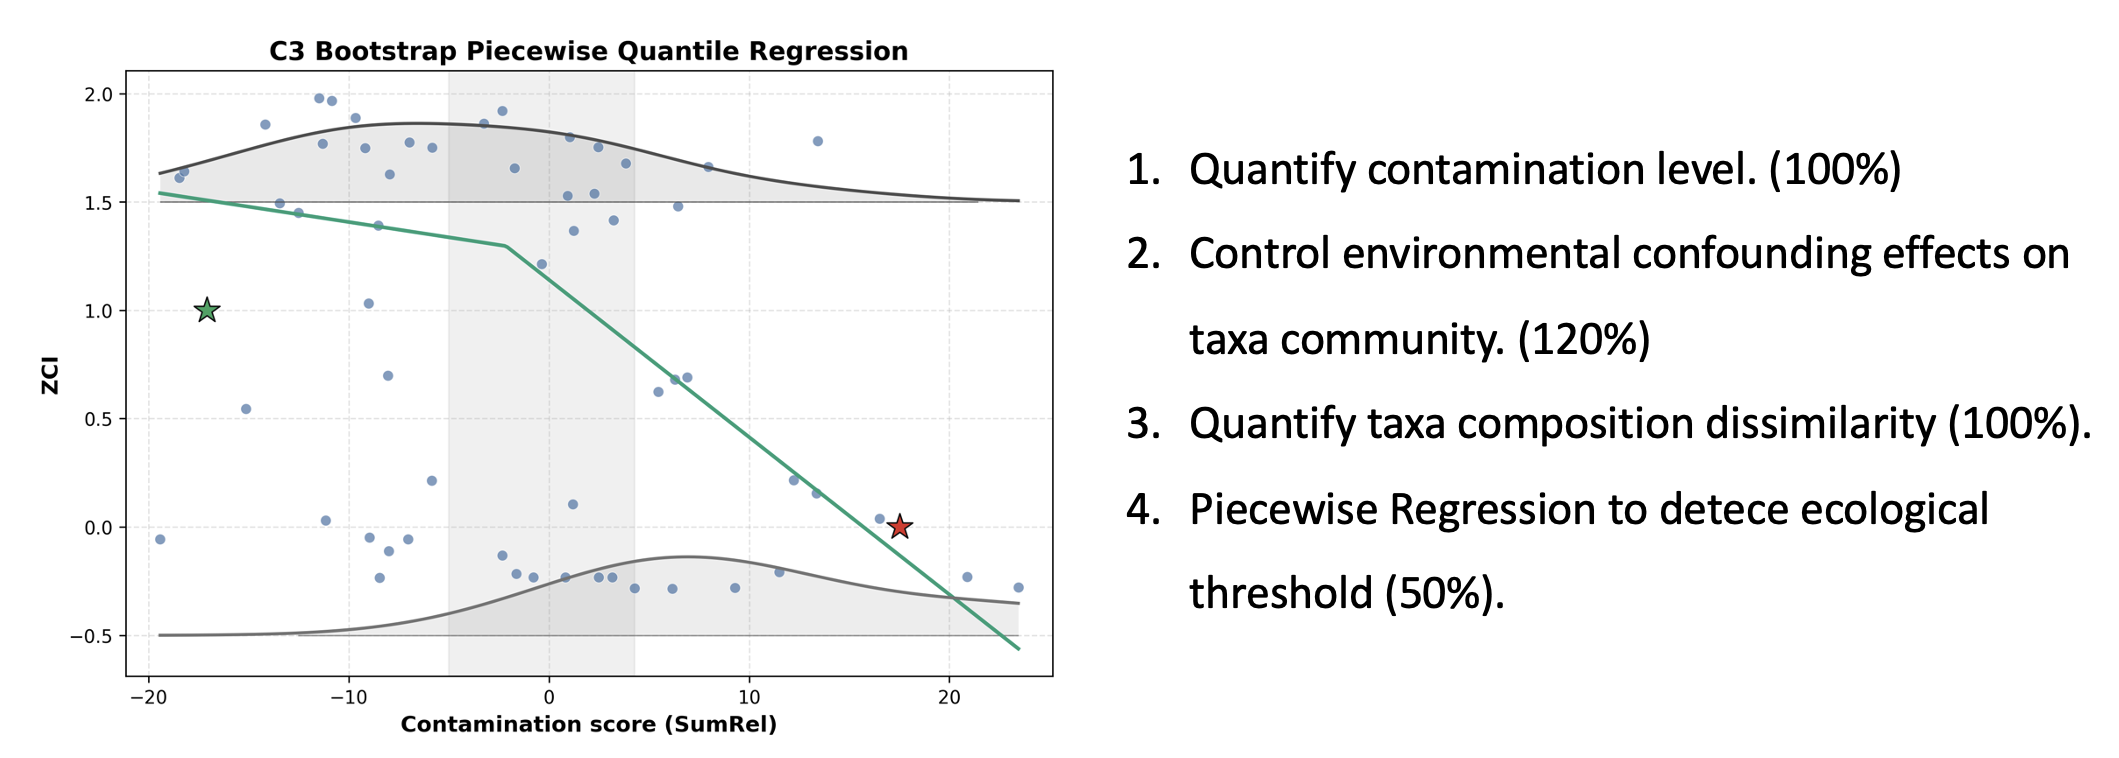
\includegraphics[width=\textwidth]
        {images/slides_1.png}
    \end{figure}
\end{frame}

% ----- Page 3 ---------------------------------------------------------
\begin{frame}{Data Source - Detroit River Zoobenthos Datasets}
    \begin{figure}
        \centering
        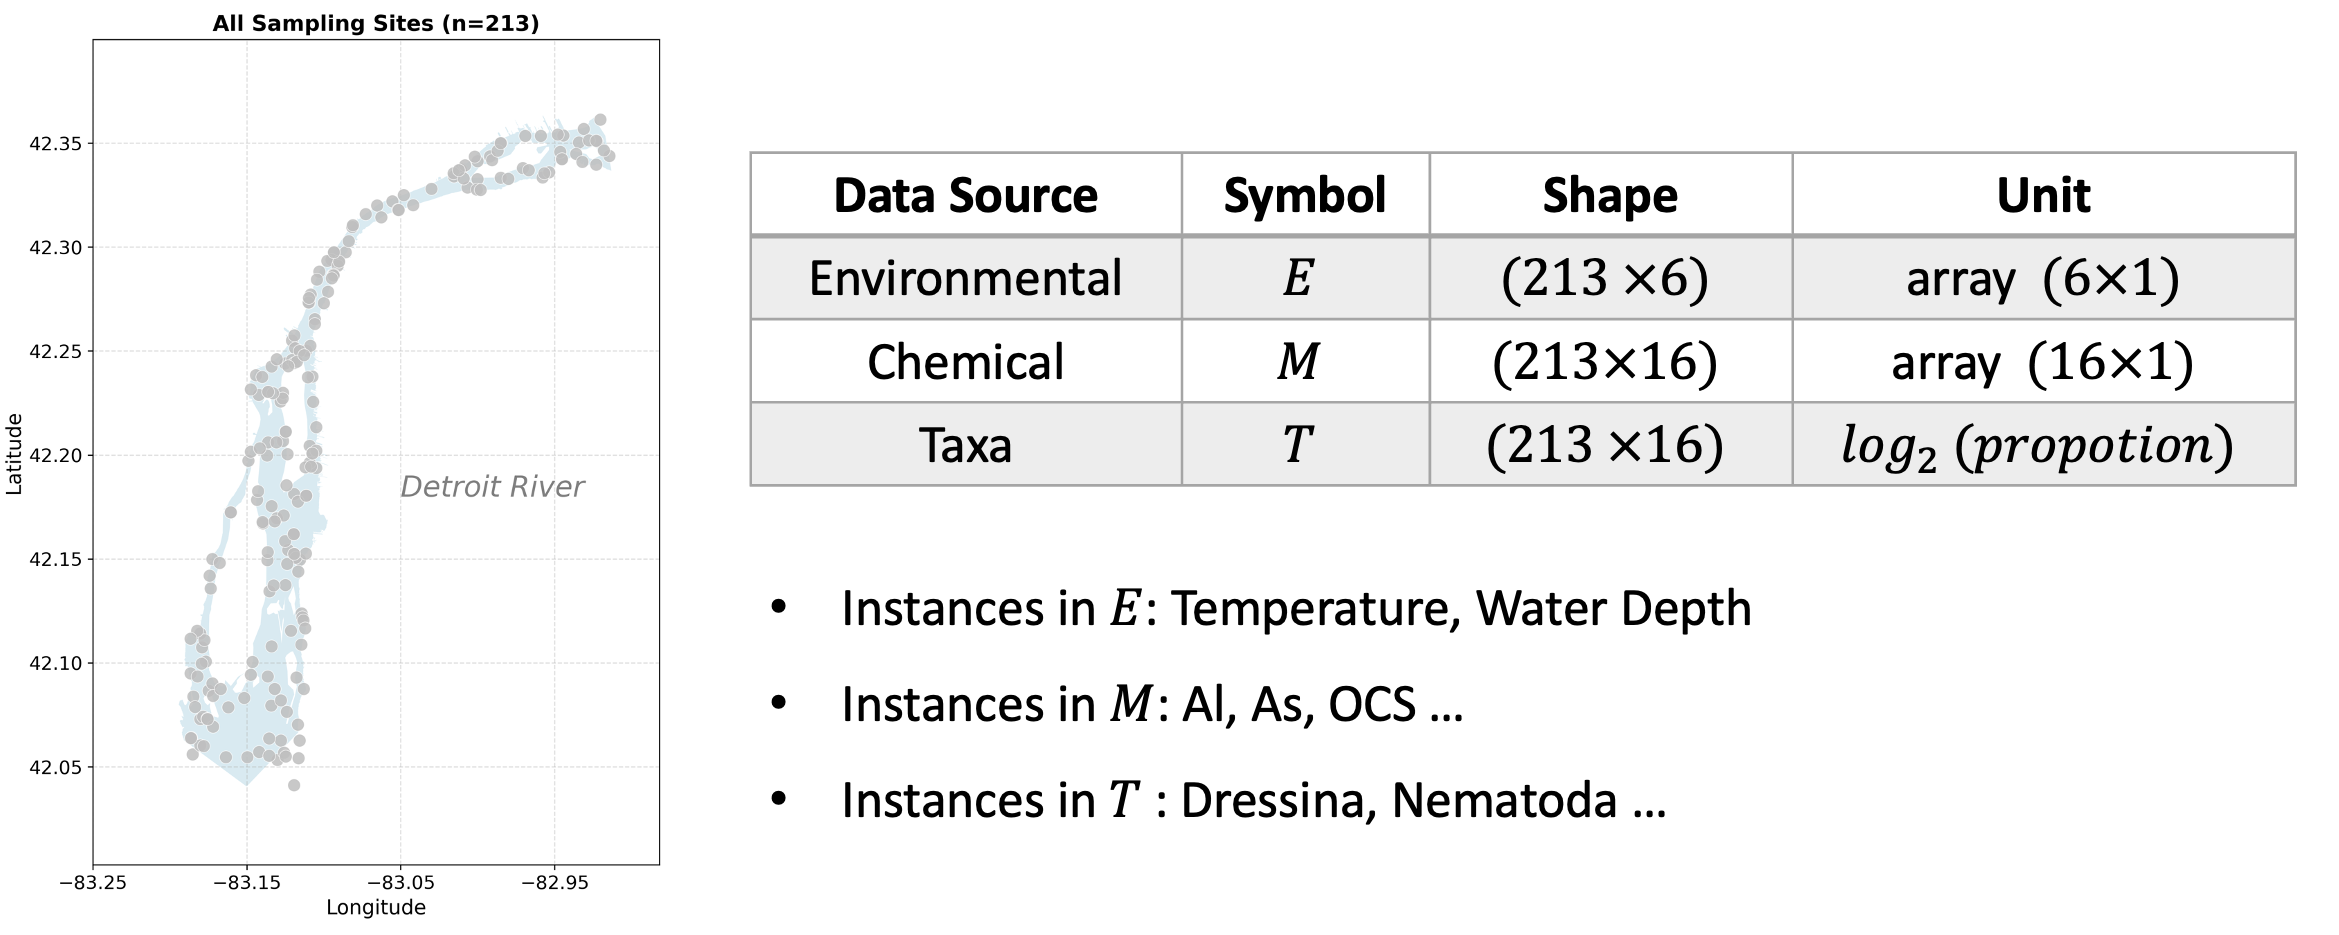
\includegraphics[width=0.9\textwidth]
        {images/slides_2.png}
    \end{figure}
    The datasets were initially organized and used by Zhang (2008),
    and provided by Dr. Jan Ciborowski for this project.
    More quality control work was done by Feng.
\end{frame}

% % ----- Page 4 ---------------------------------------------------------
\begin{frame}{Main Methodology used throughout the project}
    \begin{figure}
        \centering
        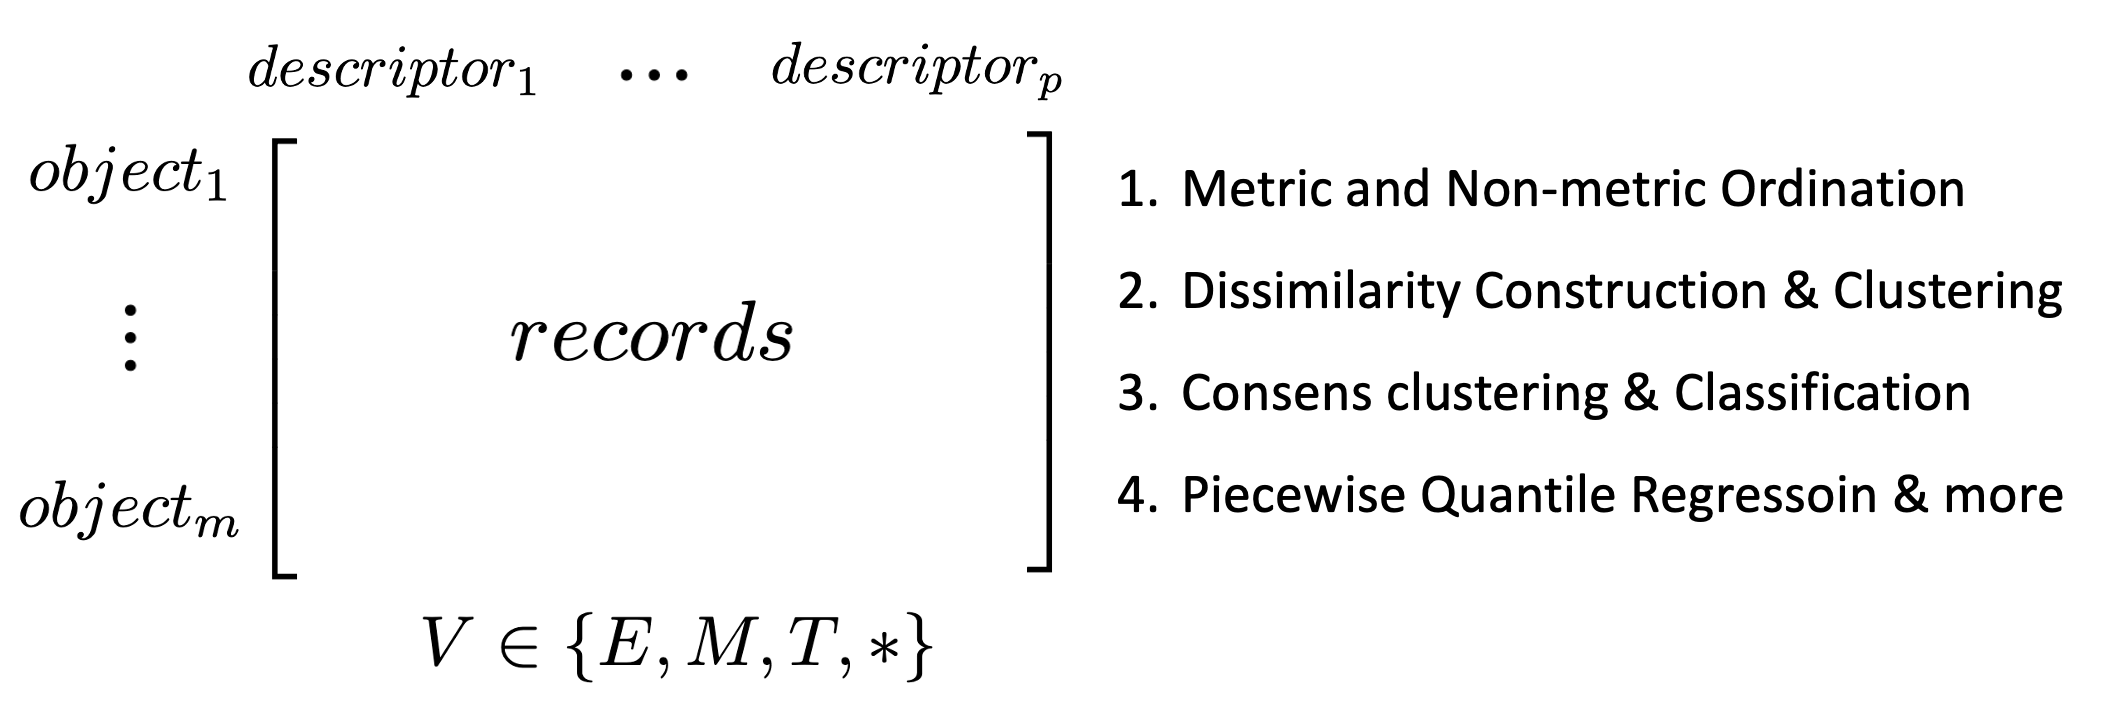
\includegraphics[width=1\textwidth]
        {images/slides_4.png}
    \end{figure}
\end{frame}

% ----- Page 5 ---------------------------------------------------------
\begin{frame}{Quantify Contamination Level through PCA on $M_{213 \times 16}$}
\[
\mathbf{M}_{213 \times 16}
\xrightarrow{\log(1+x)\;+\;\mathrm{cor}}
\mathbf{Cor}_{16 \times 16}
\xrightarrow{\mathrm{PCA,\ rotation,\ and\ selection}}
\mathbf{L}_{16 \times 5}
\]

\begin{figure}
    \centering
    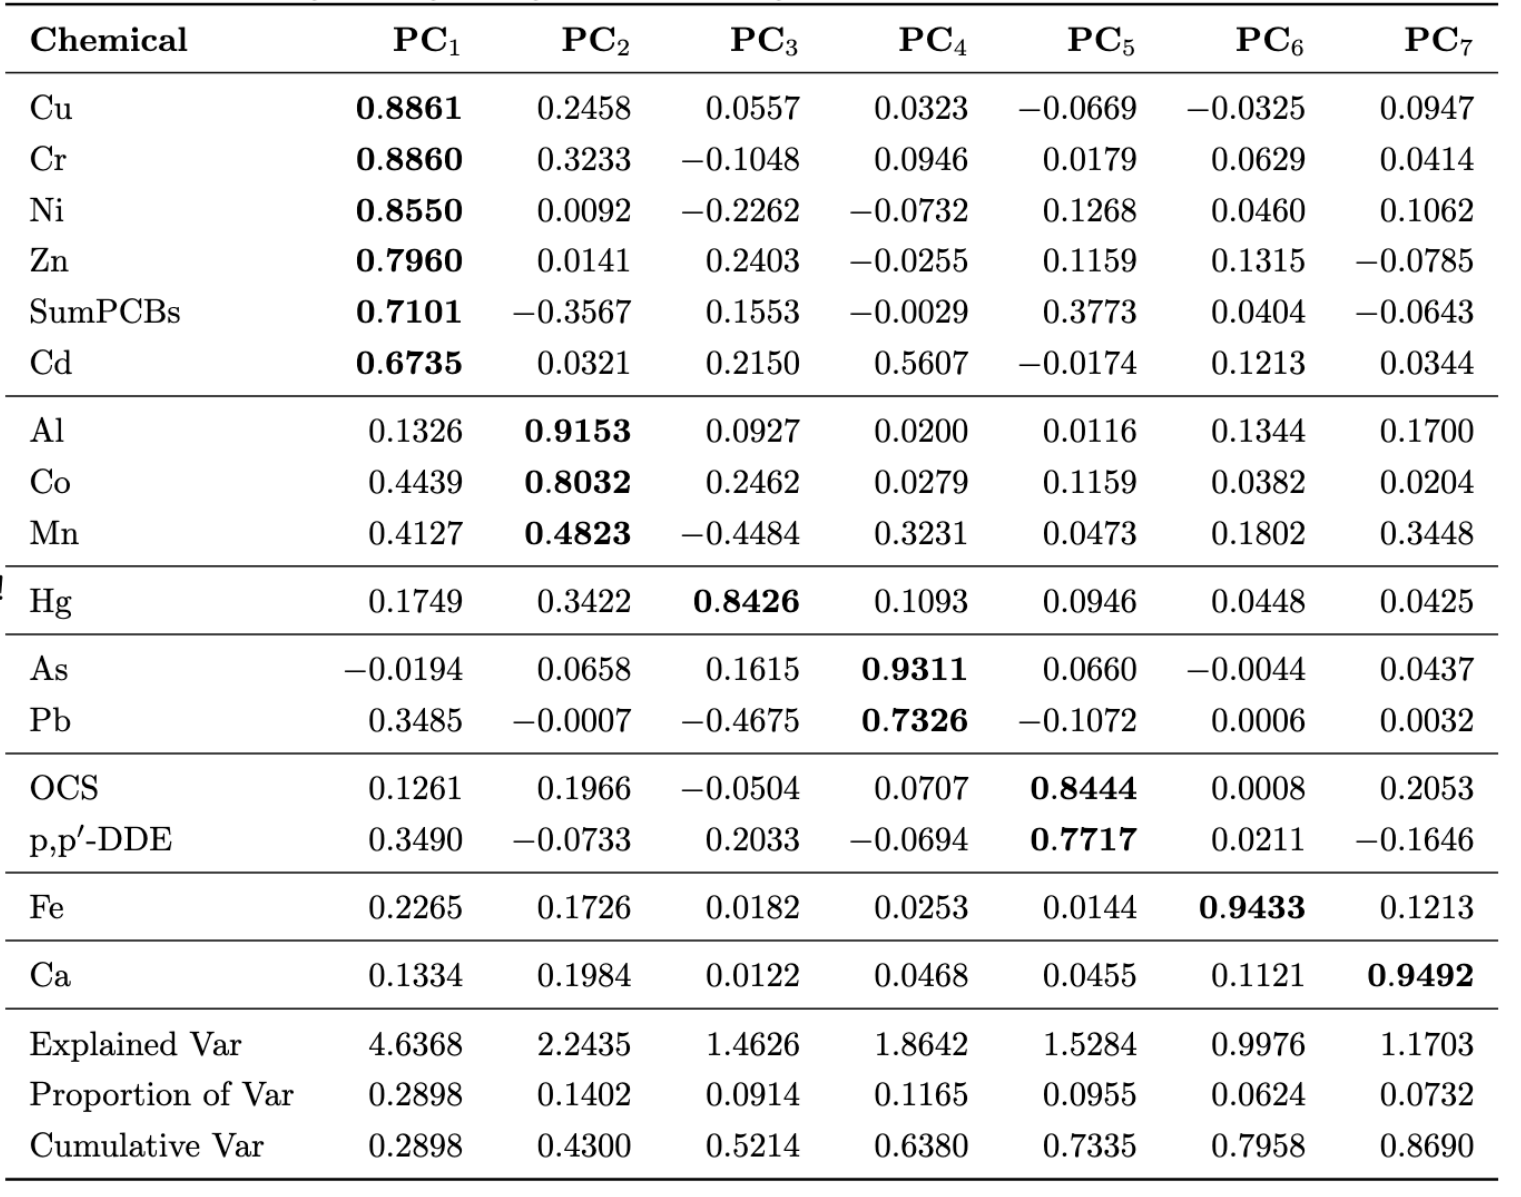
\includegraphics[width=0.5\textwidth]
    {images/loadings2.png}
\end{figure}

\end{frame}

\begin{frame}{Quantify Contamination Level through PCA on $M_{213 \times 16}$}
\[
\mathbf{L}_{16 \times 5}
\xrightarrow{\mathbf{M}'\mathbf{L}}
\mathbf{S}_{213 \times 5}
\xrightarrow{\mathbf{S}_{213\times5} \mathbf{1}_{5\times1}}
\mathbf{C}_{213 \times 1}
\]
\begin{figure}
    \centering
    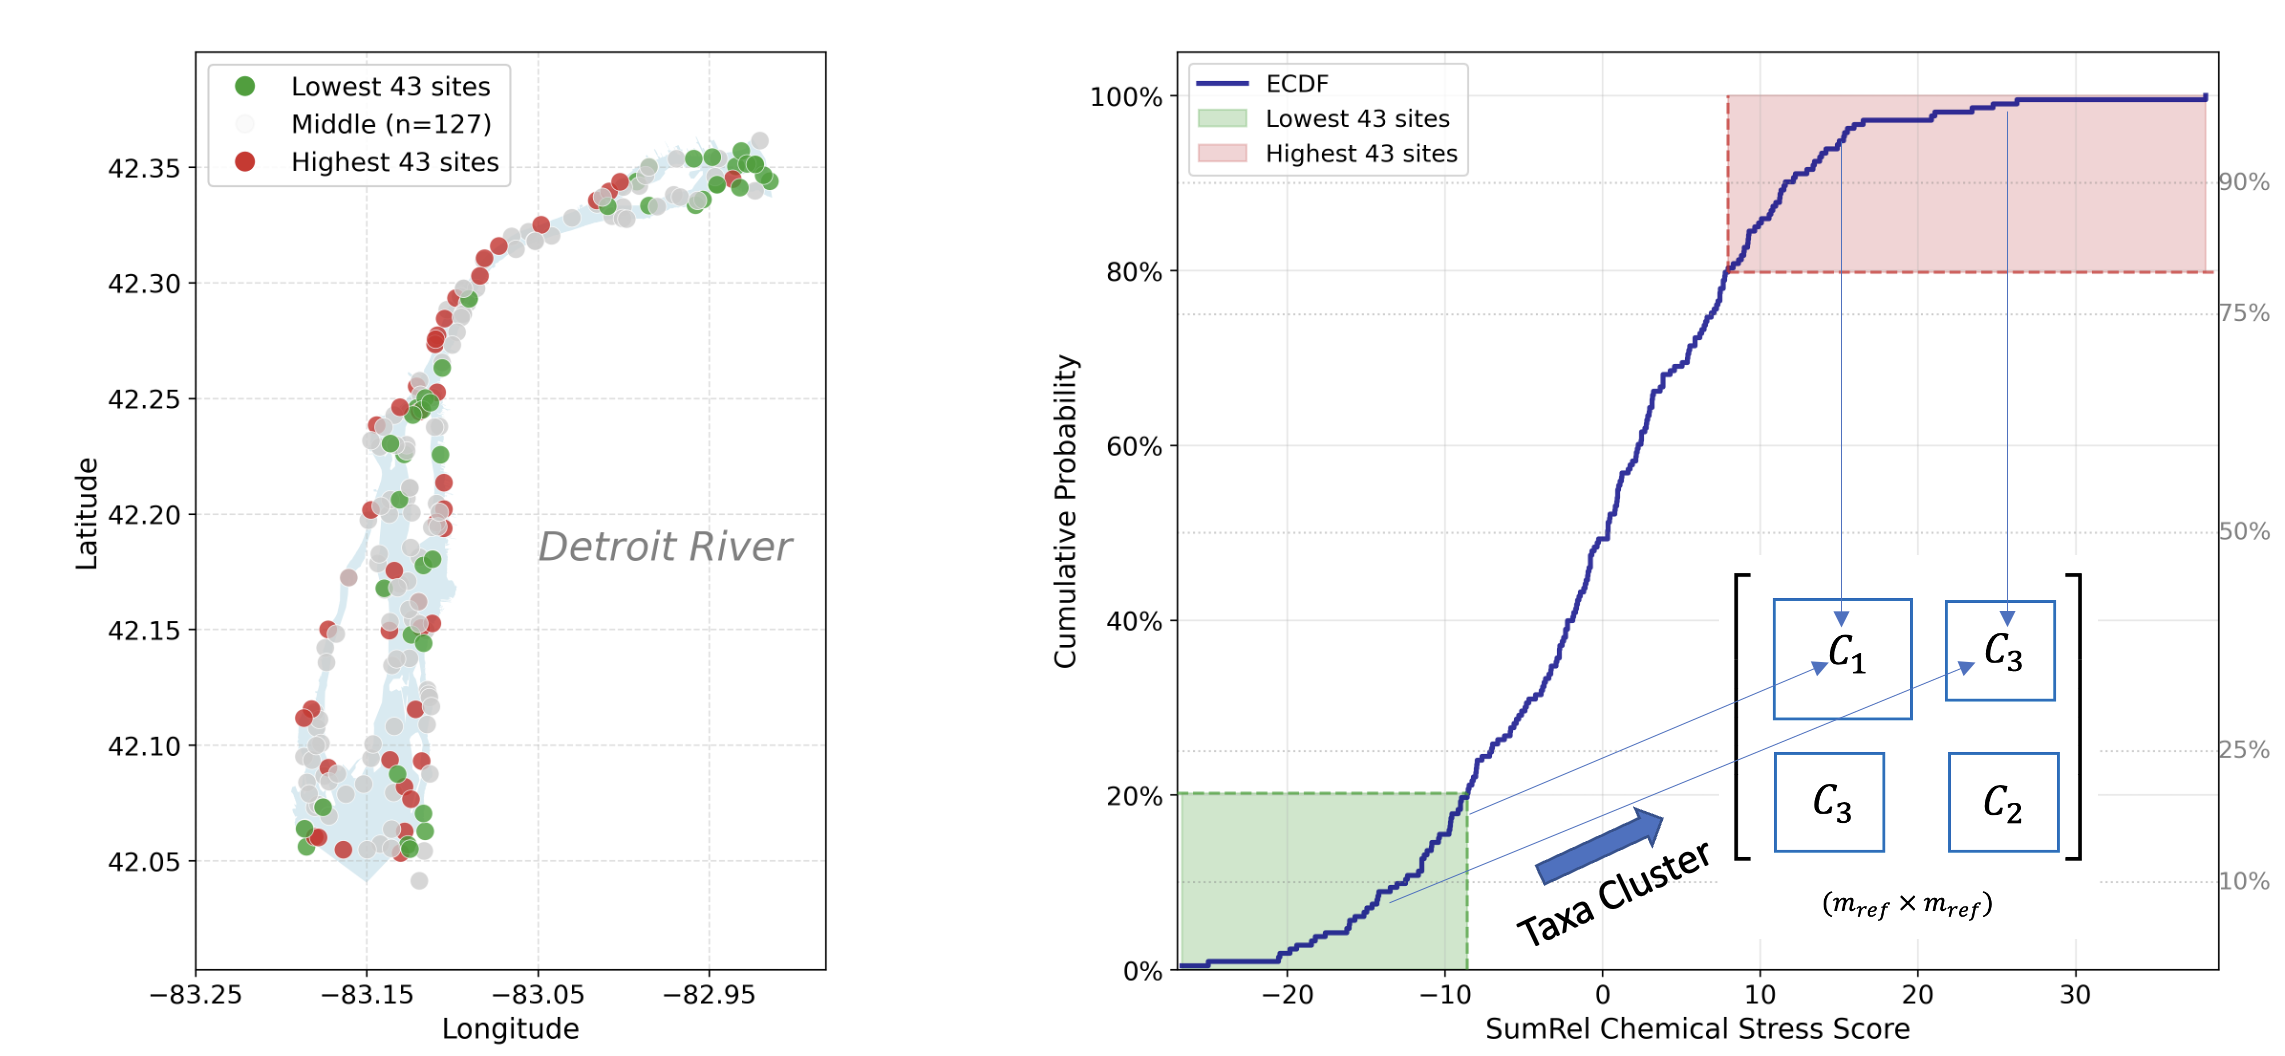
\includegraphics[width=0.7\textwidth]
    {images/slide5.png}
    \caption{Contamination Scores (additive view) of sites in the Detroit River}
\end{figure}
\end{frame}

\begin{frame}{Test the Hypothesis of Least-Contamination effects on Community Composition of these Sites}

\begin{figure}
    \centering
    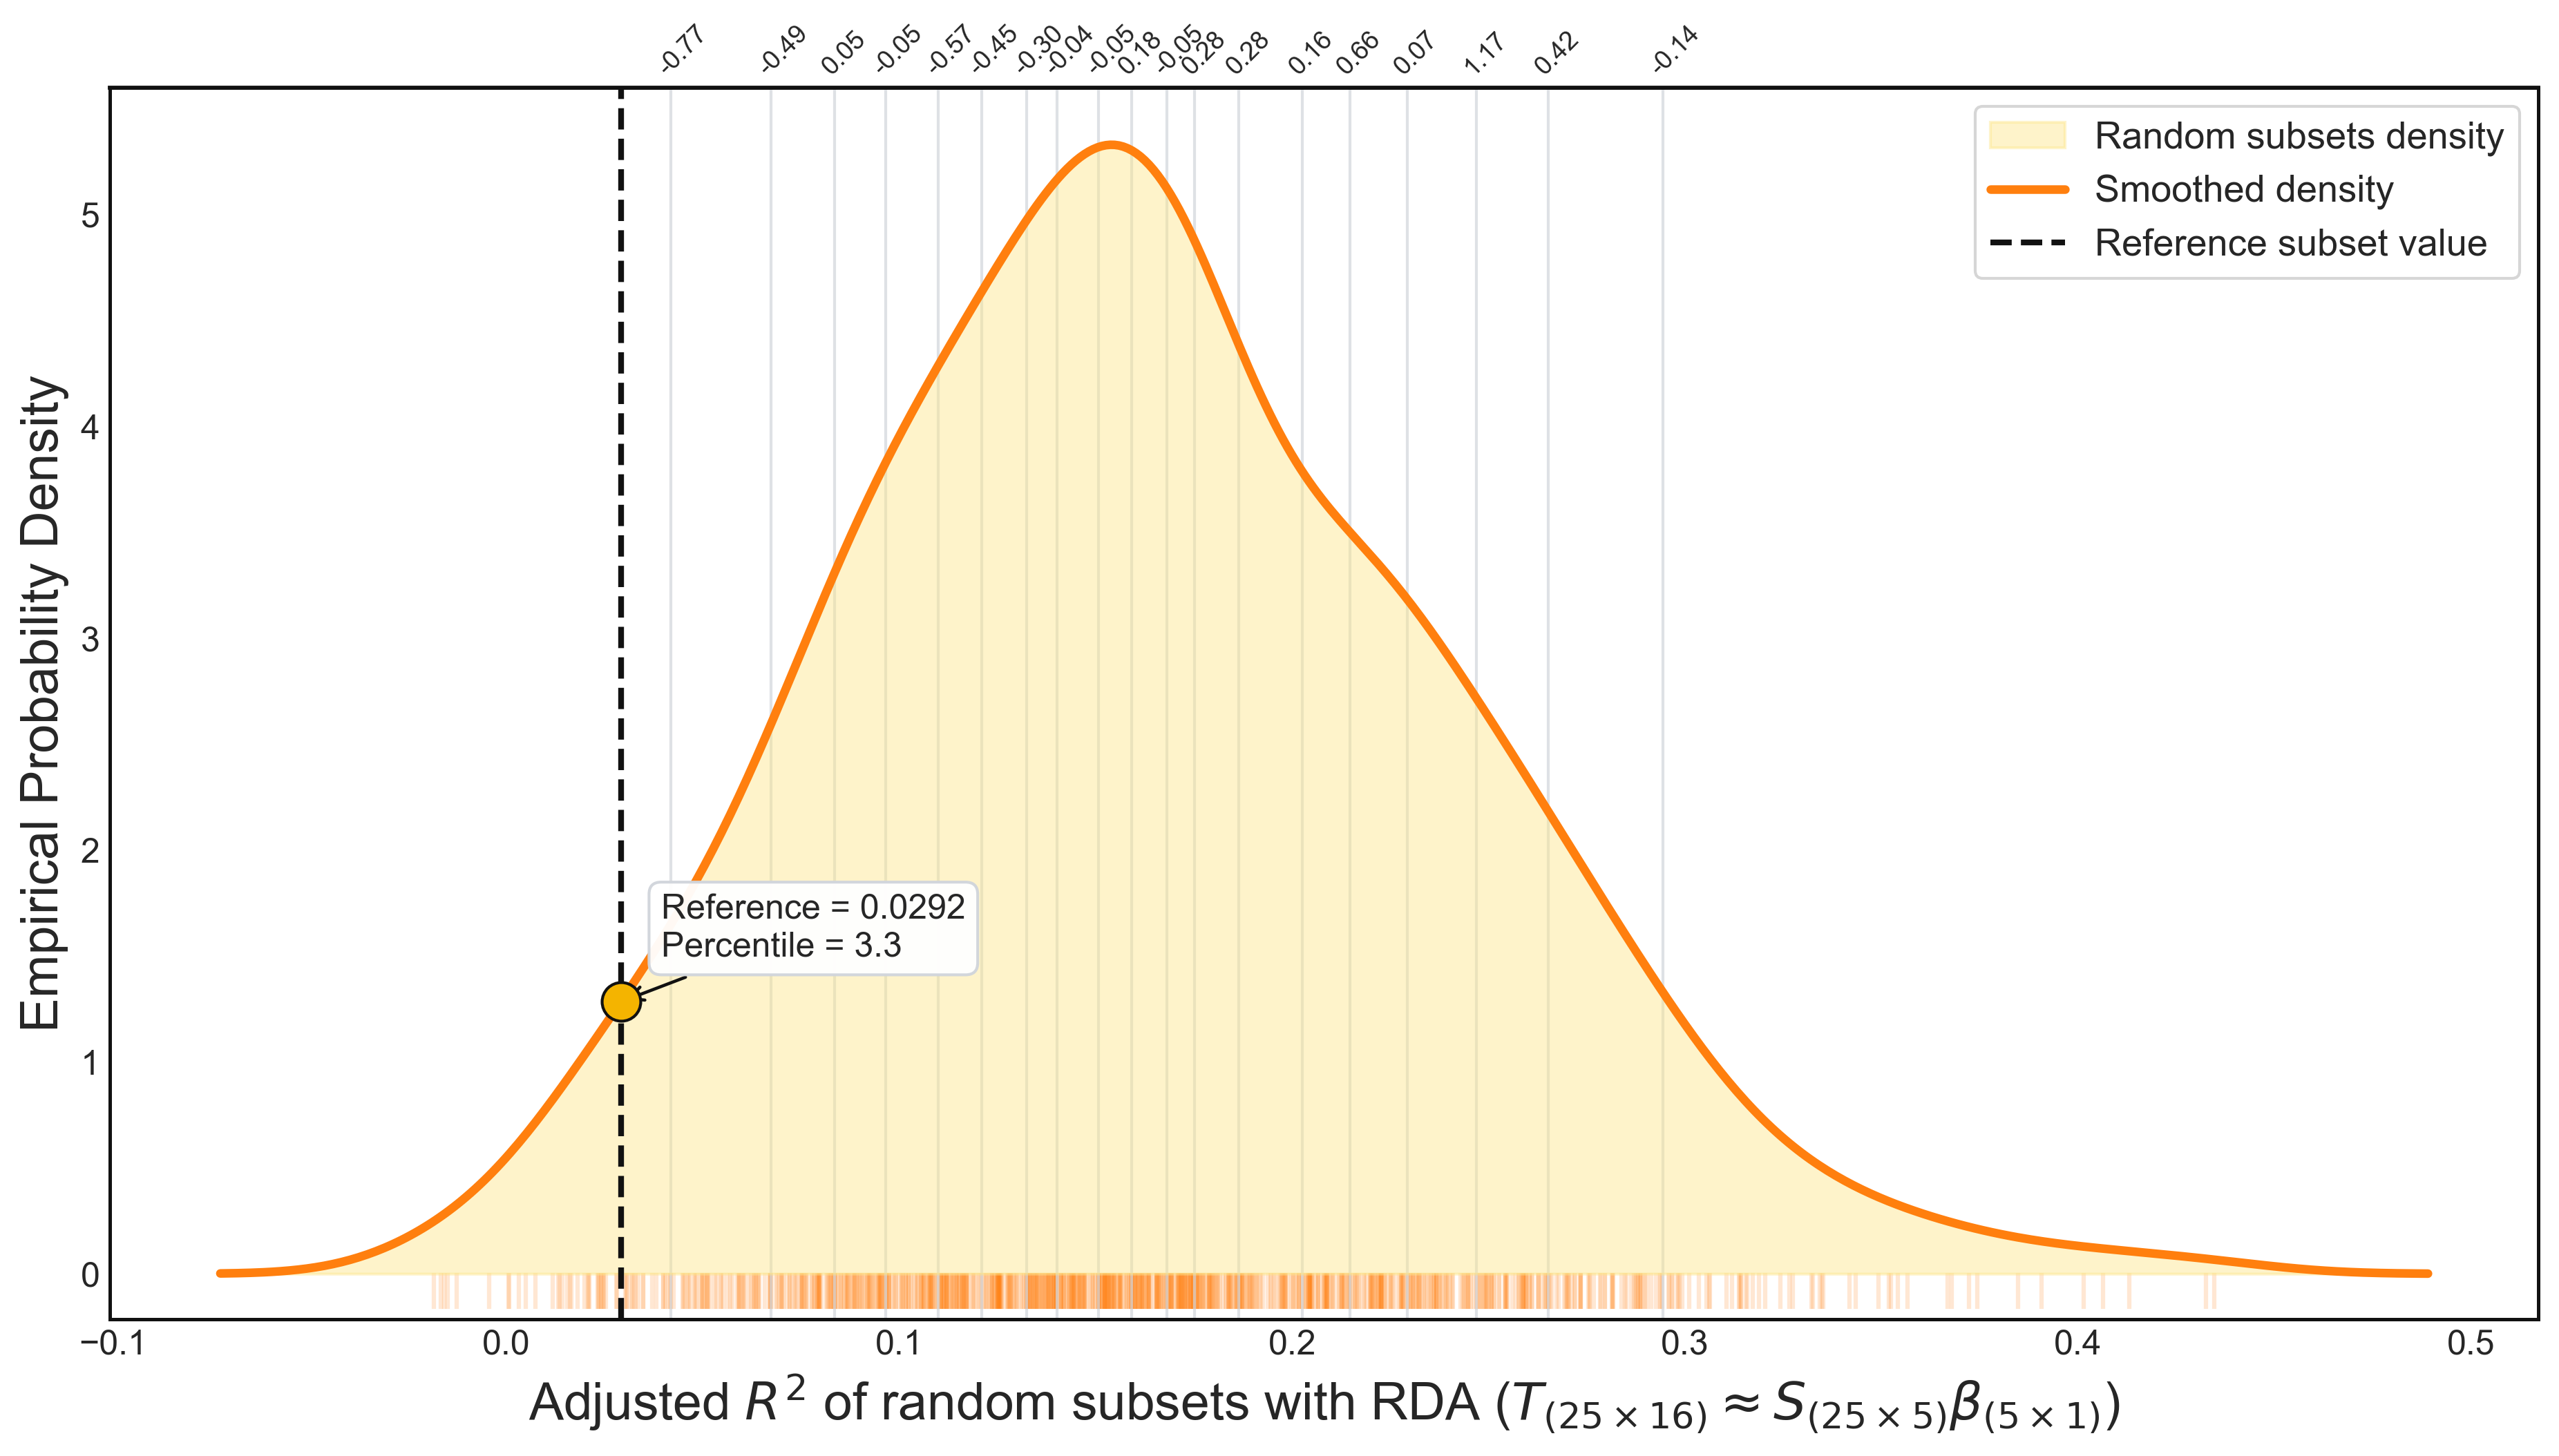
\includegraphics[width=0.65\textwidth]
    {images/test_h0.png}
    \caption{Empirical distribution of $\bar R^2$
 from 1000 randomly resampled 62-site subsets and the average contamination scores of every 50 sets around similar $\bar R^2$}
\end{figure}

\end{frame}

% page 6
\begin{frame}{Define Expected Community Types in Least Contamination Affected $m_{ref}$ sites}
    \begin{figure}
        \centering
        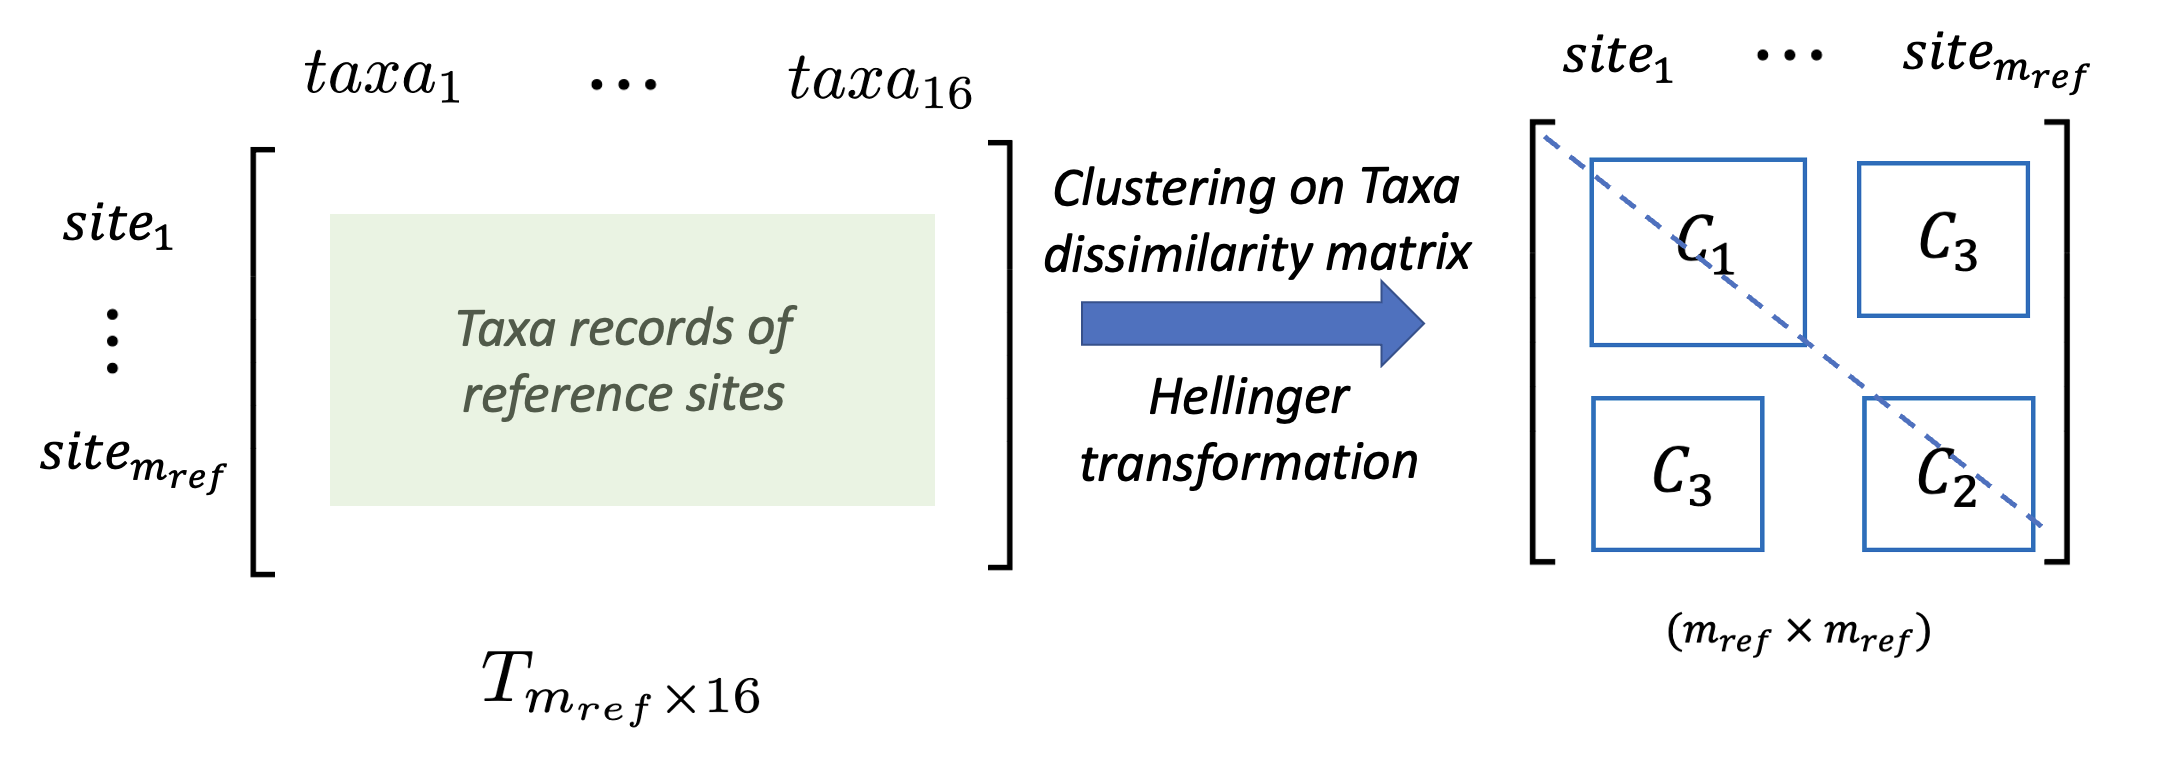
\includegraphics[width=0.9\textwidth]
        {images/slide_6_2.png}
        \caption{Idea of using $m_{ref}$ sites to define natural taxa clusters}
        \end{figure}
\end{frame}

% page 7 
\begin{frame}{Community Types through Wards Clustering with Hellinger Distance of Taxa Abundance}
    \begin{figure}
        \centering
        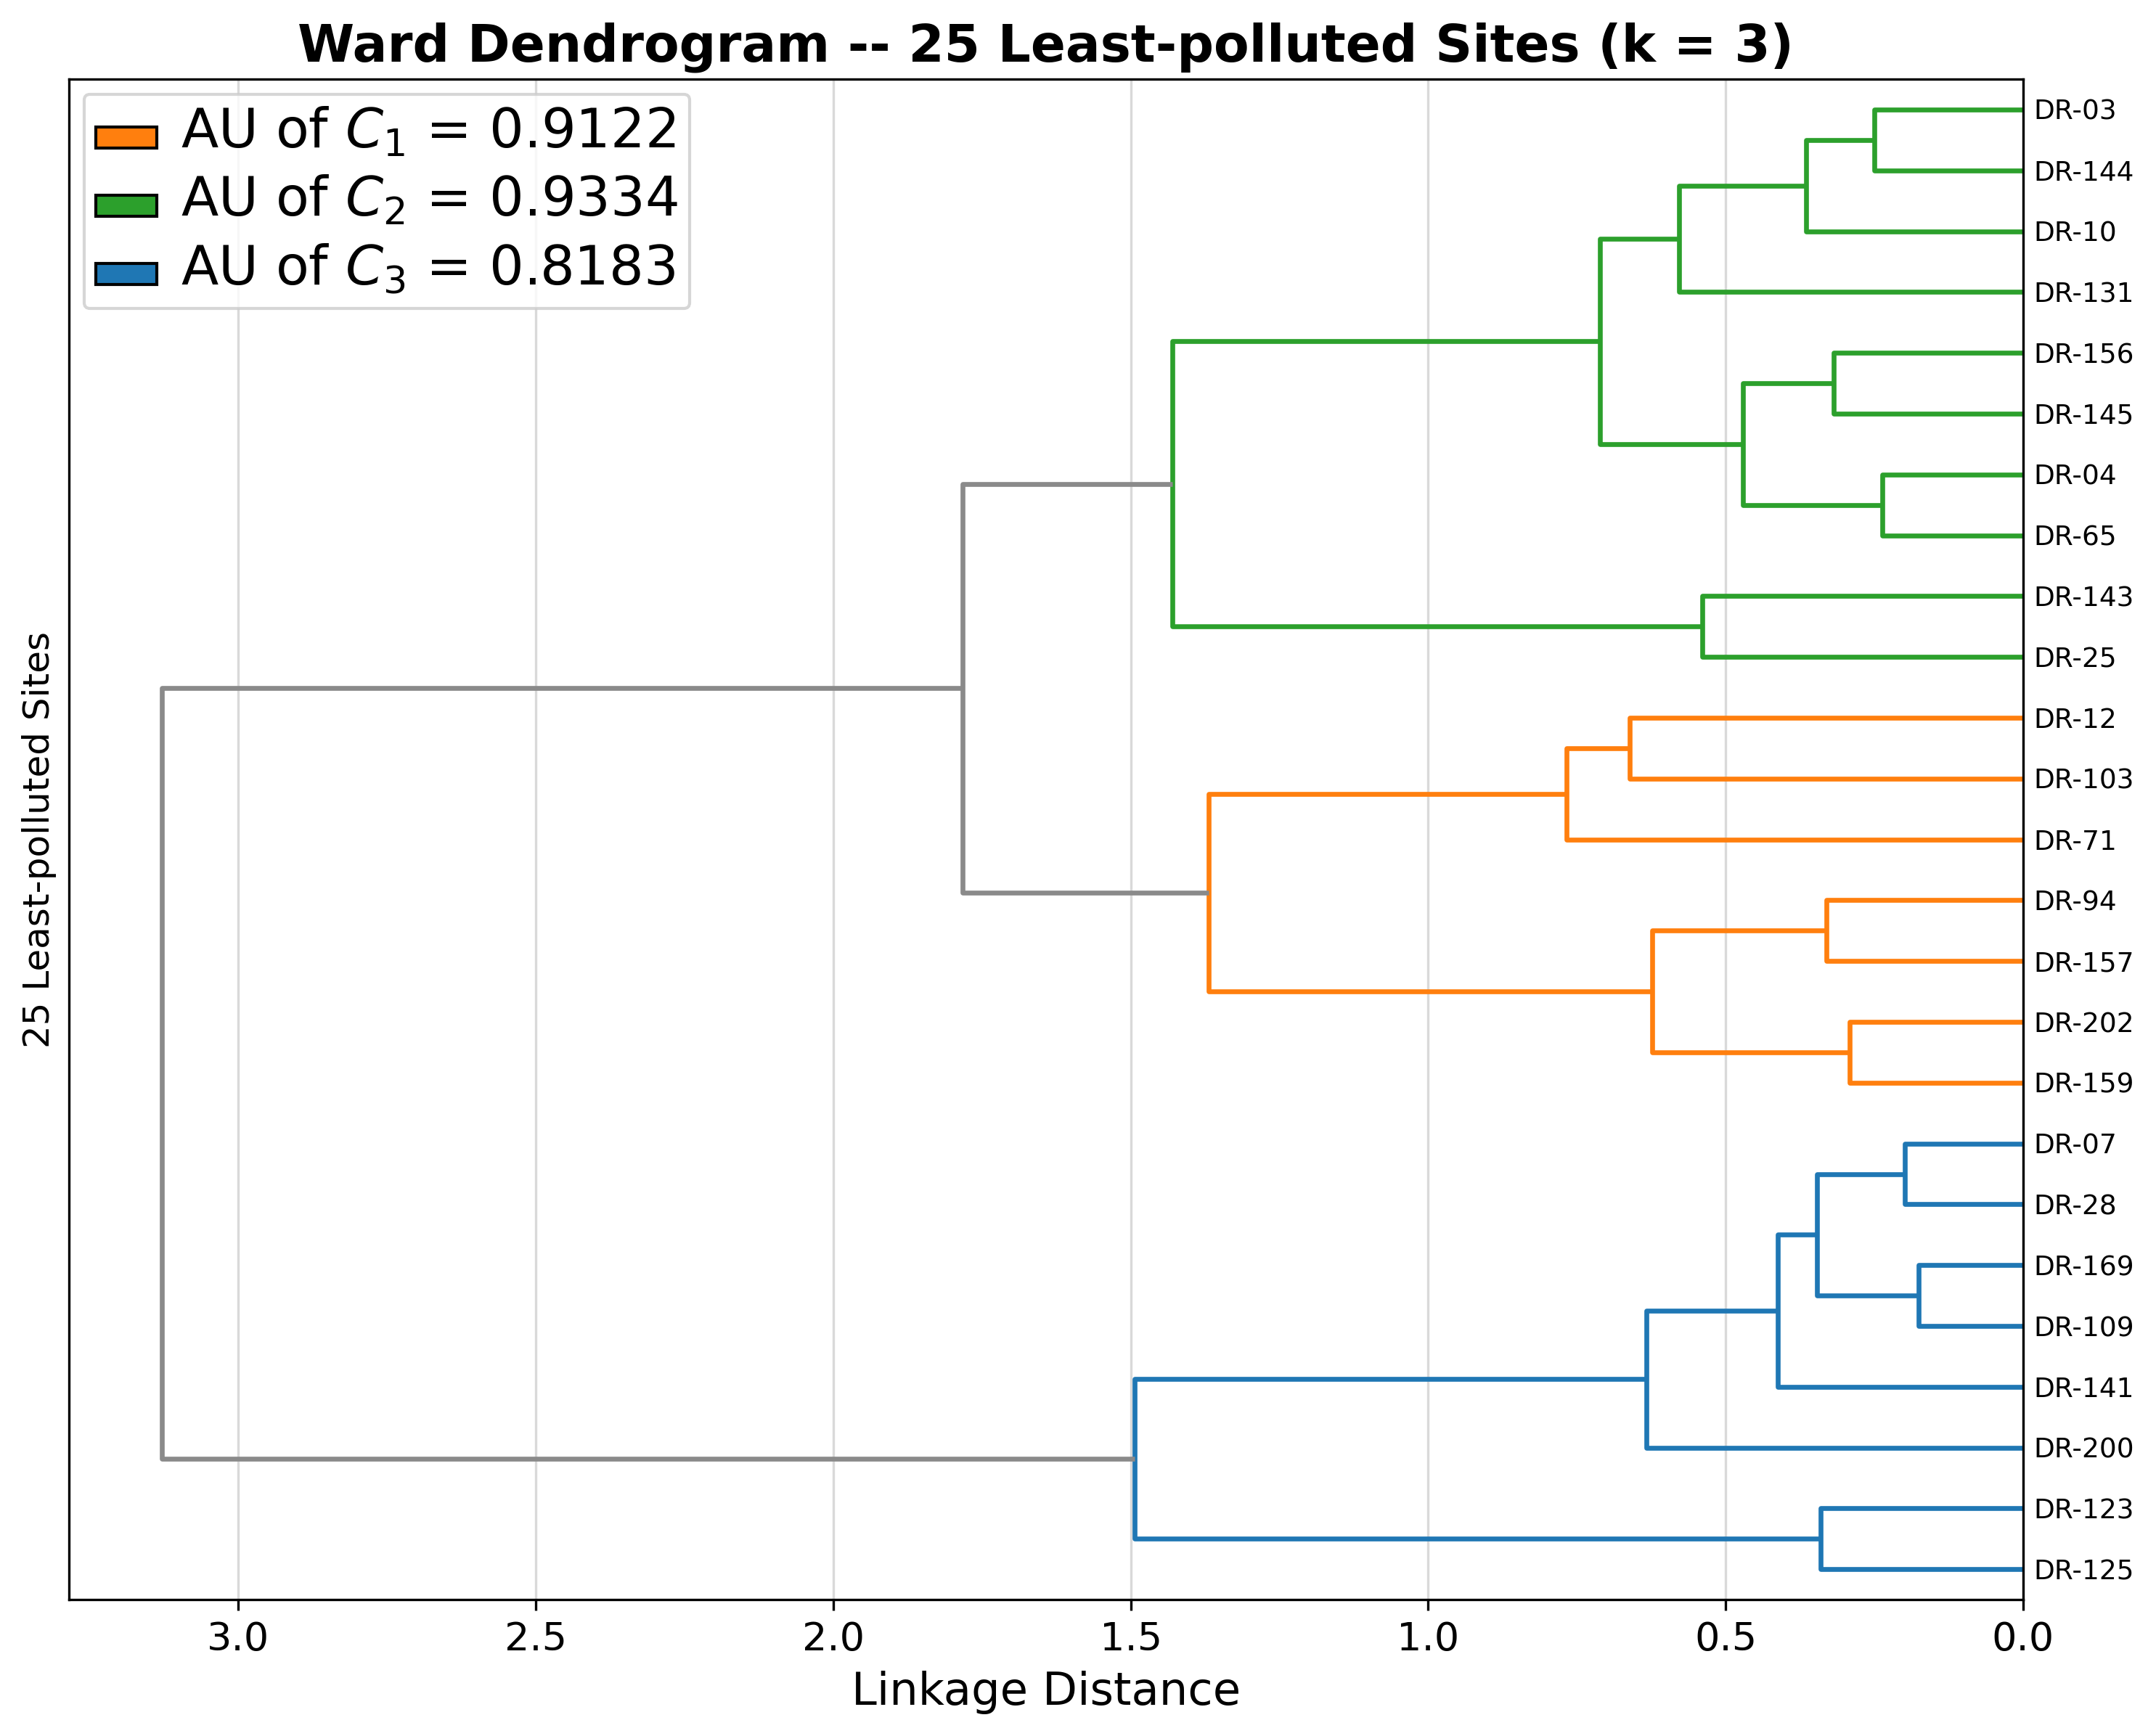
\includegraphics[width=0.55\textwidth]
        {images/slides_7.png}
        \caption{Idea of using $m_{ref}$ sites to define natural taxa clusters}
    \end{figure}
\end{frame}

% page 8
\begin{frame}{Searching Concordant Sites with Supportive Environmental Profiles}
    \begin{figure}
        \centering
        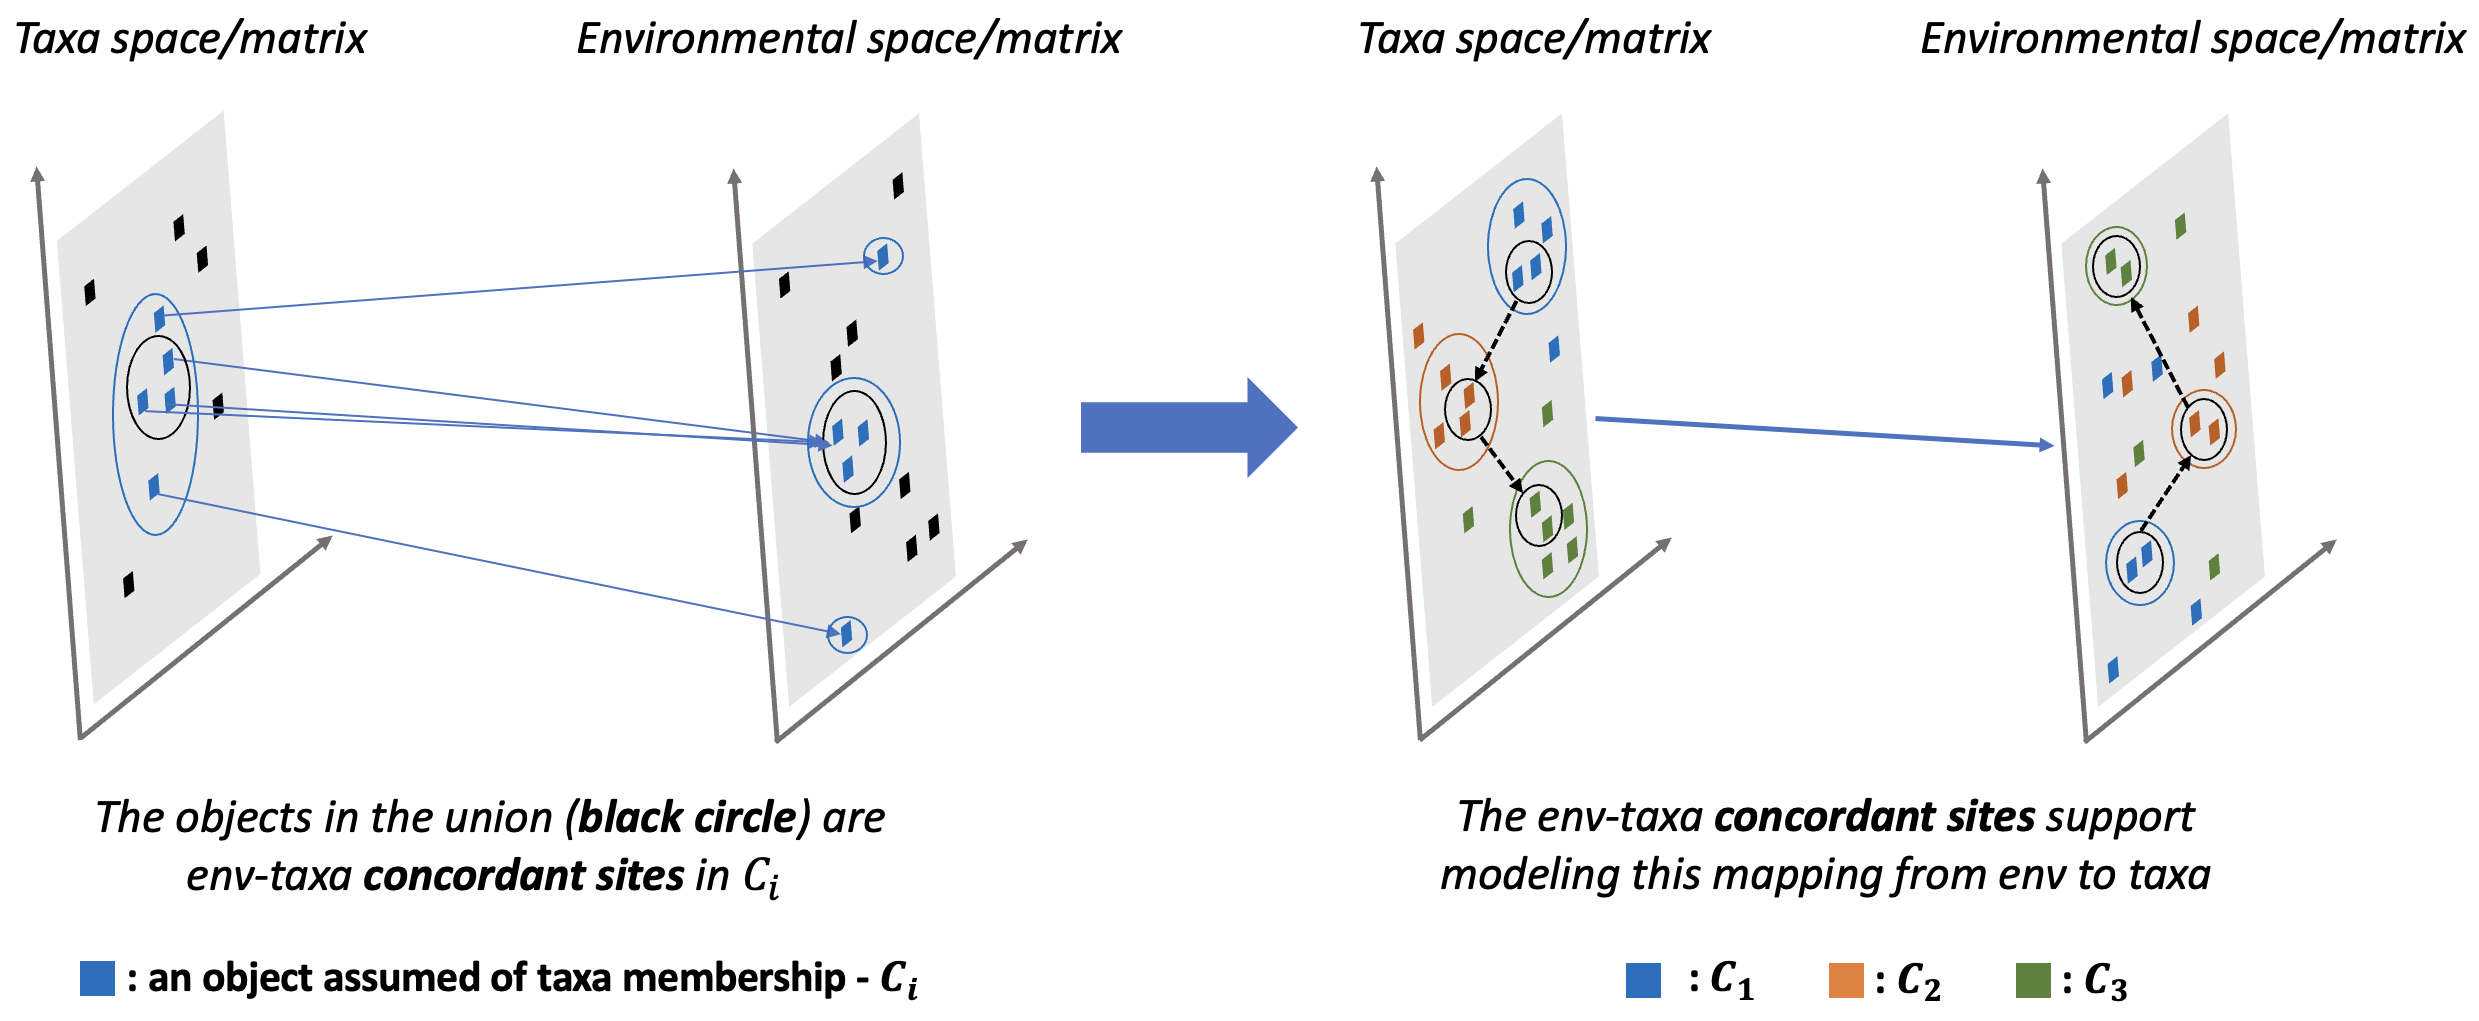
\includegraphics[width=0.9\textwidth]
        {images/slides_8.png}
        \caption{Idea of cross-checking sites with defined community types over
        both taxa and environmental spaces to decide which are concordant or conflicting}
    \end{figure}
\end{frame}


% page 9
\begin{frame}{Consensus Clustering with Defined Clusters to Detect Concordant Sites}
    \begin{figure}
        \centering
        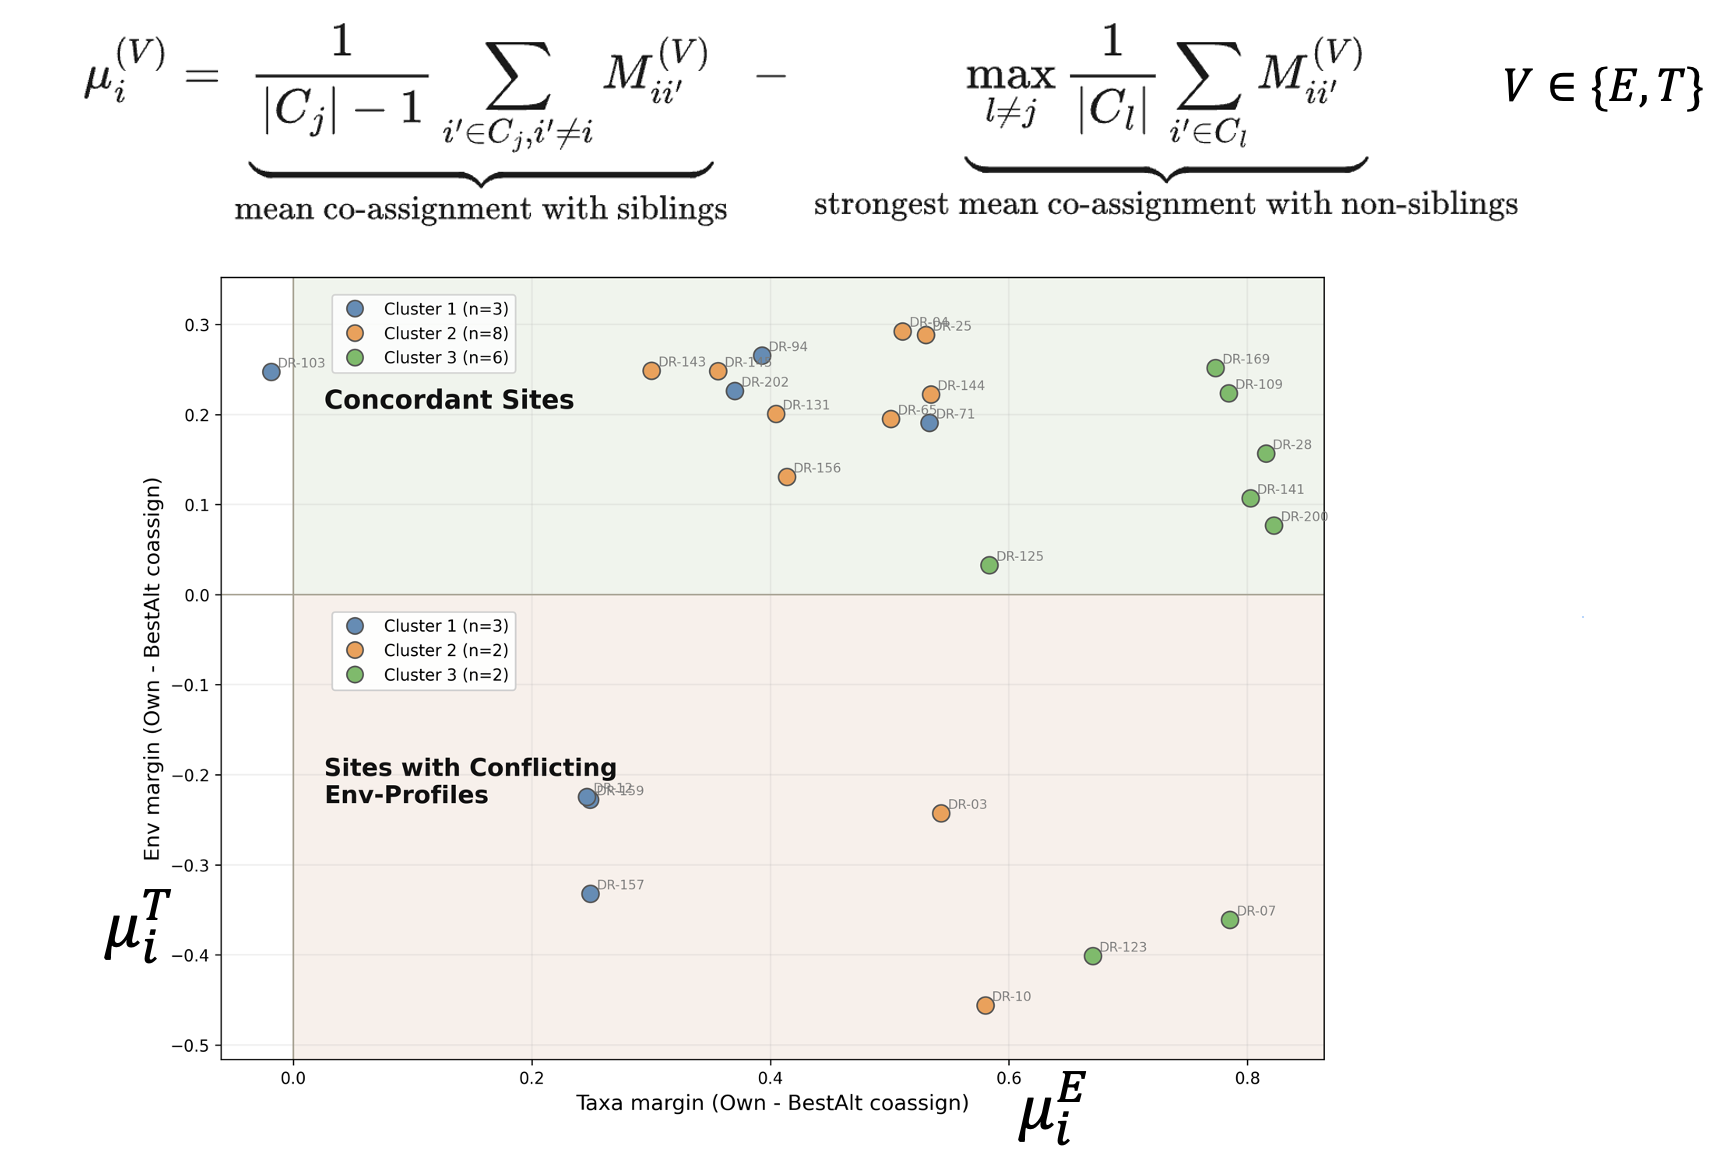
\includegraphics[width=0.75\textwidth]
        {images/slides_9.png}
    \end{figure}
\end{frame}


% page 10
\begin{frame}{Stratified Confusion Matrix of LDA Classifier trained on concordant sites}
    \begin{figure}
        \centering
        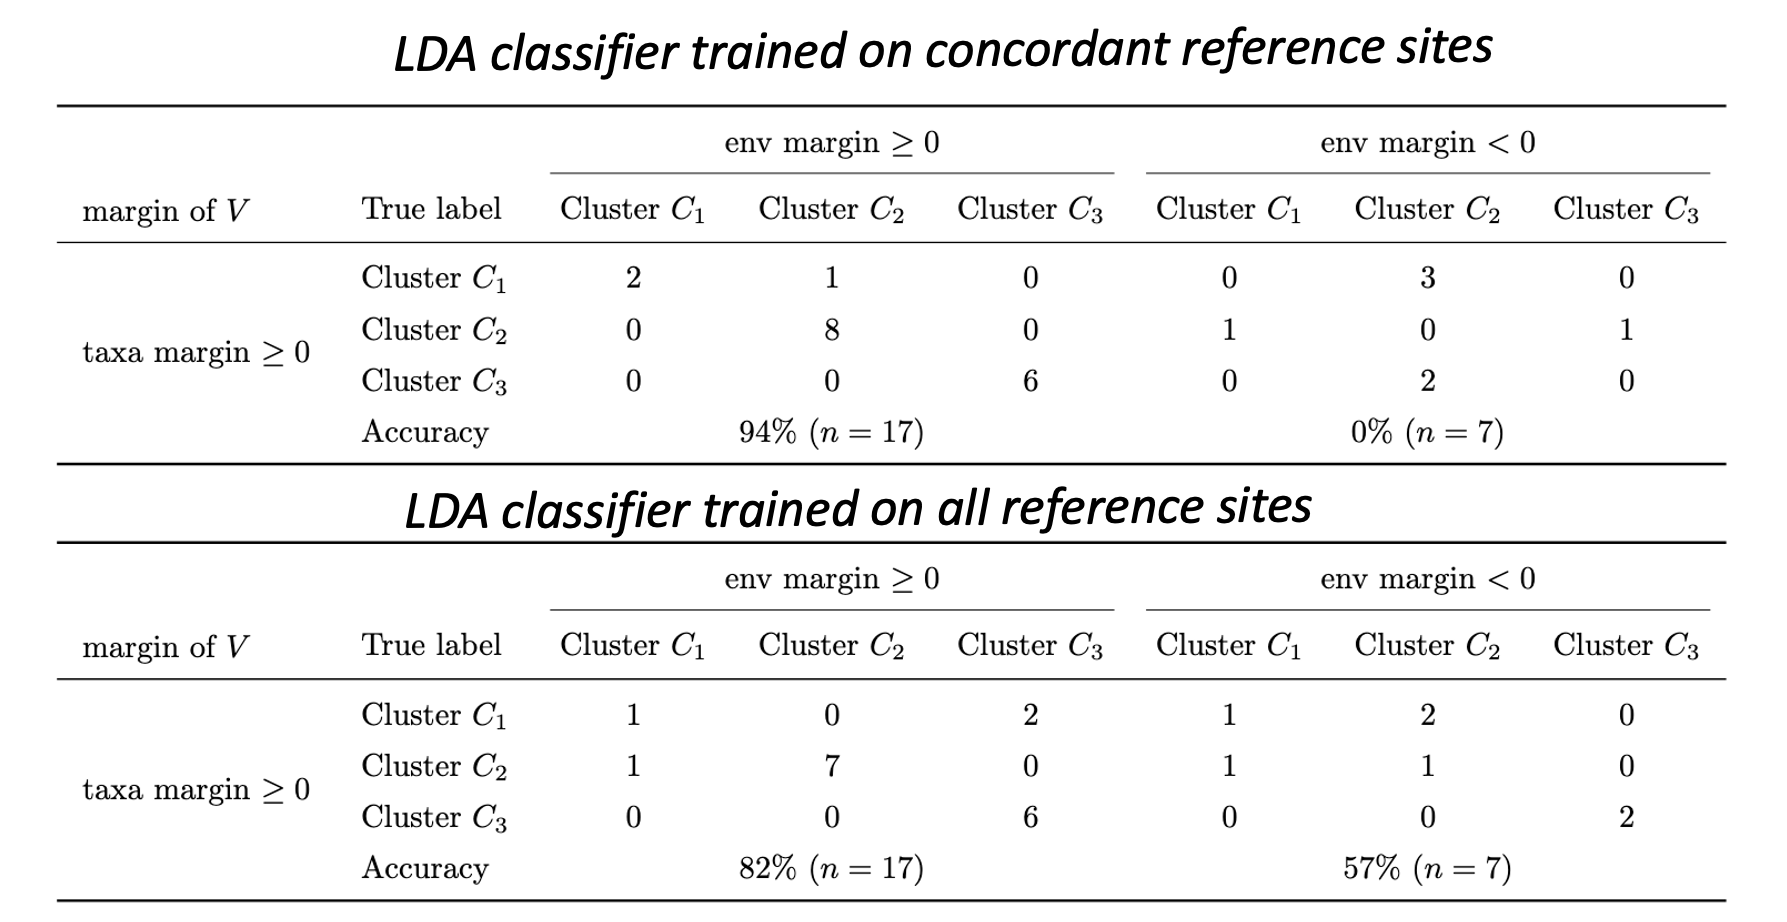
\includegraphics[width=0.85\textwidth]
        {images/slides_10.png}
    \end{figure}
\end{frame}


% page 11
\begin{frame}{Random-split Cross-validation of LDA Classifier trained on concordant sites}
    \begin{figure}
        \centering
        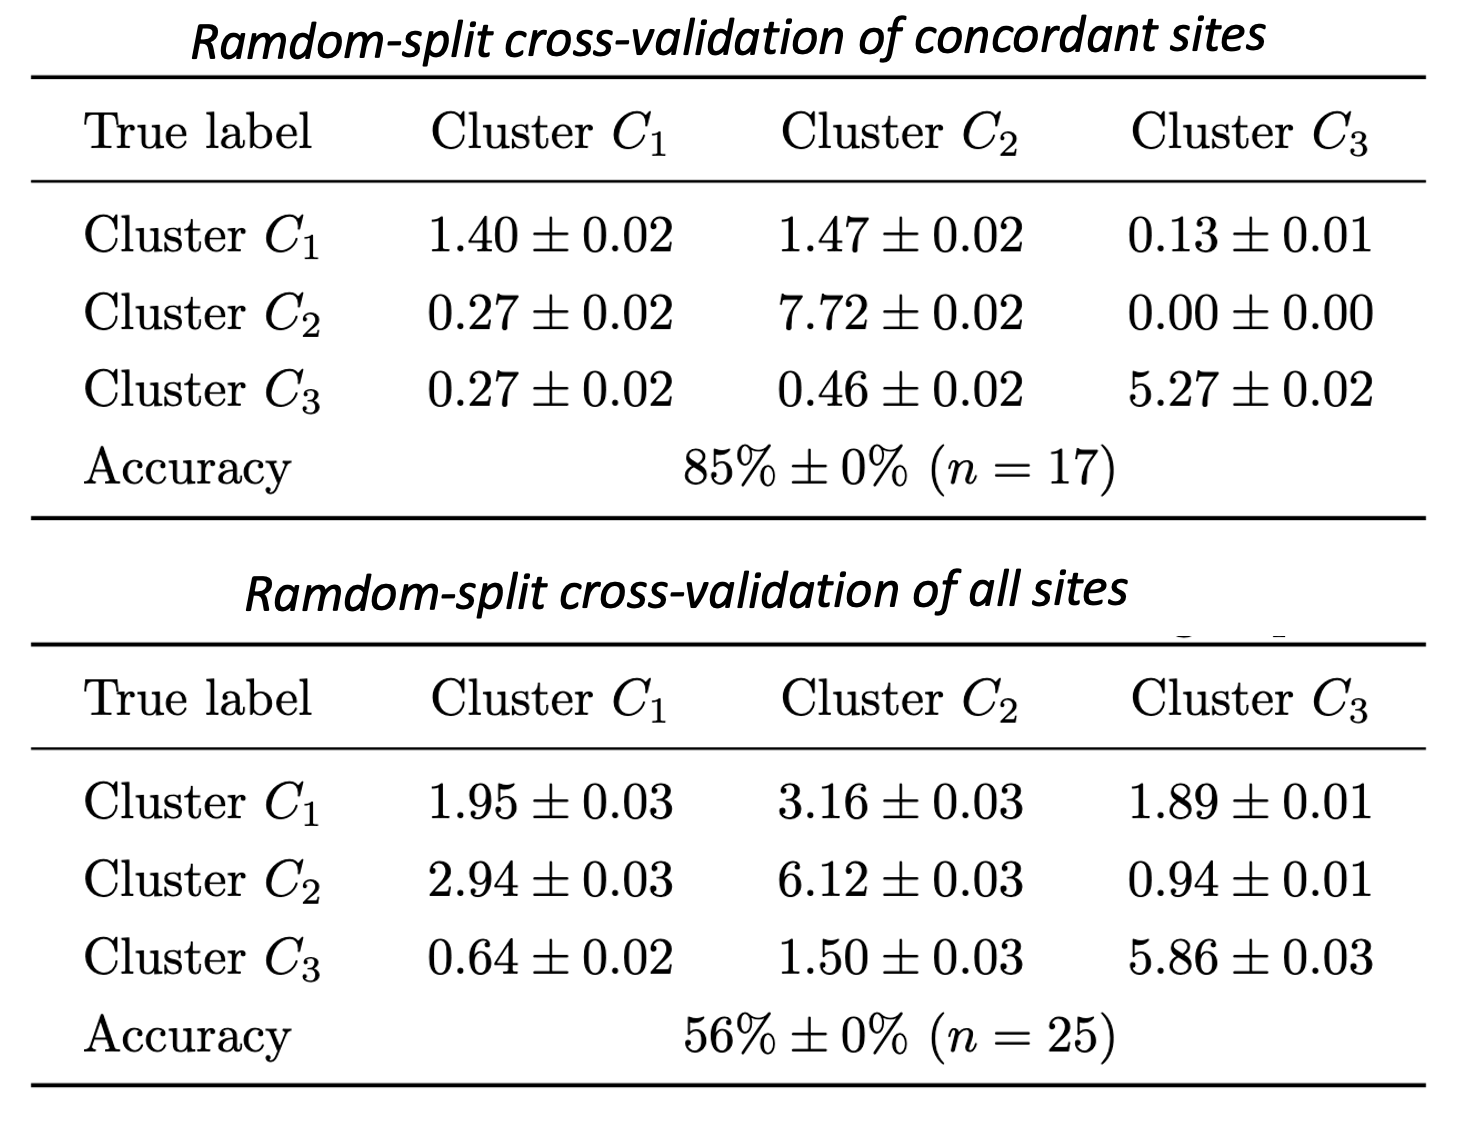
\includegraphics[width=0.60\textwidth]
        {images/slides_11.png}
    \end{figure}
\end{frame}


% page 12
\begin{frame}{Classifier Interprets the Environmental Profiles into Community Types}
    \begin{figure}
        \centering
        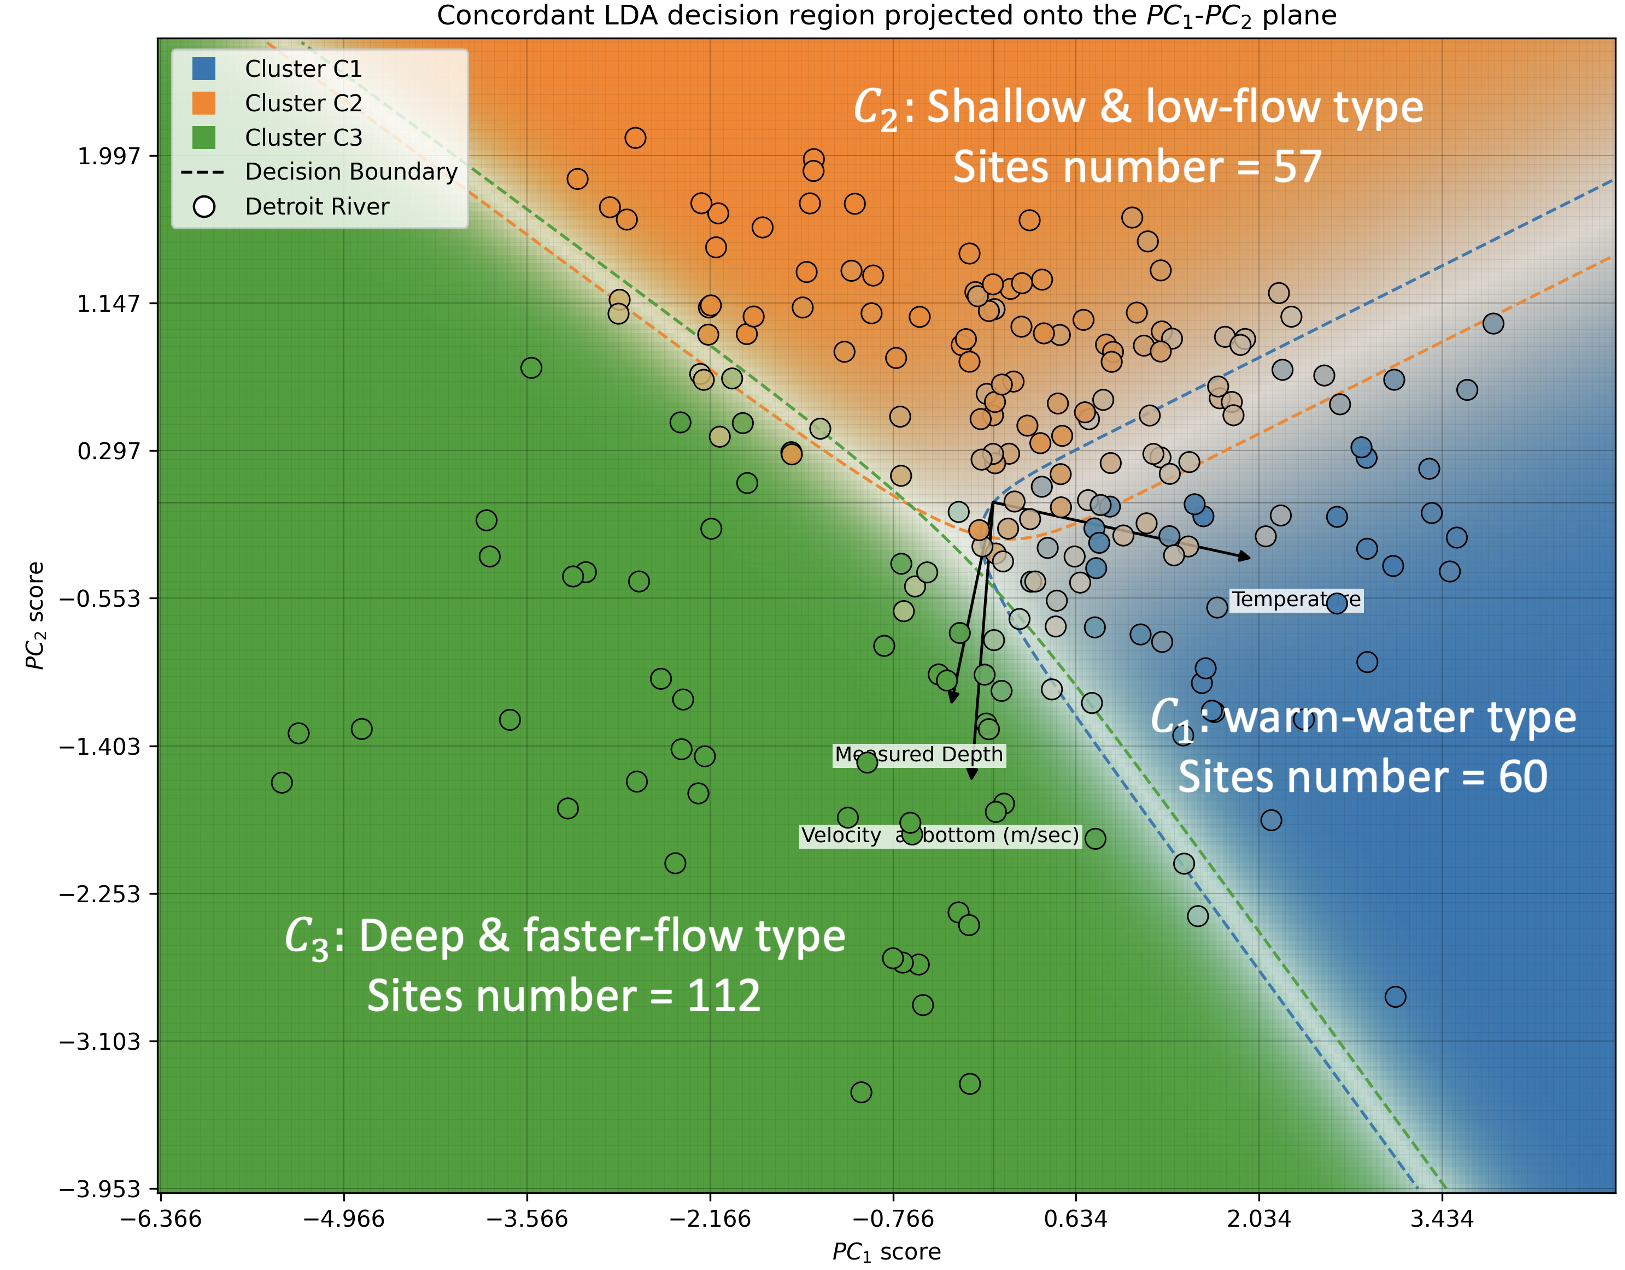
\includegraphics[width=0.63\textwidth]
        {images/slides_12_4.png}
    \end{figure}
\end{frame}

% page 13
\begin{frame}{Community dissimilarity measure: Bray-Curtis Dissimilarity and NMDS}

\[
\begin{aligned}
\mathbf{T}_{m_{c_i} \times 16}
&\xrightarrow{+\ \mathrm{poles}}
\mathbf{T}^{+}_{(m_{c_i}+2) \times 16}
\xrightarrow{\mathrm{Bray\text{-}Curtis}}
\mathbf{D}^{BC}_{(m_{c_i}+2) \times (m_{c_i}+2)}
&\xrightarrow{\mathrm{NMDS}}
\mathbf{Y}_{(m_{c_i}+2) \times q}
\end{aligned}
\]

\begin{figure}
    \centering
    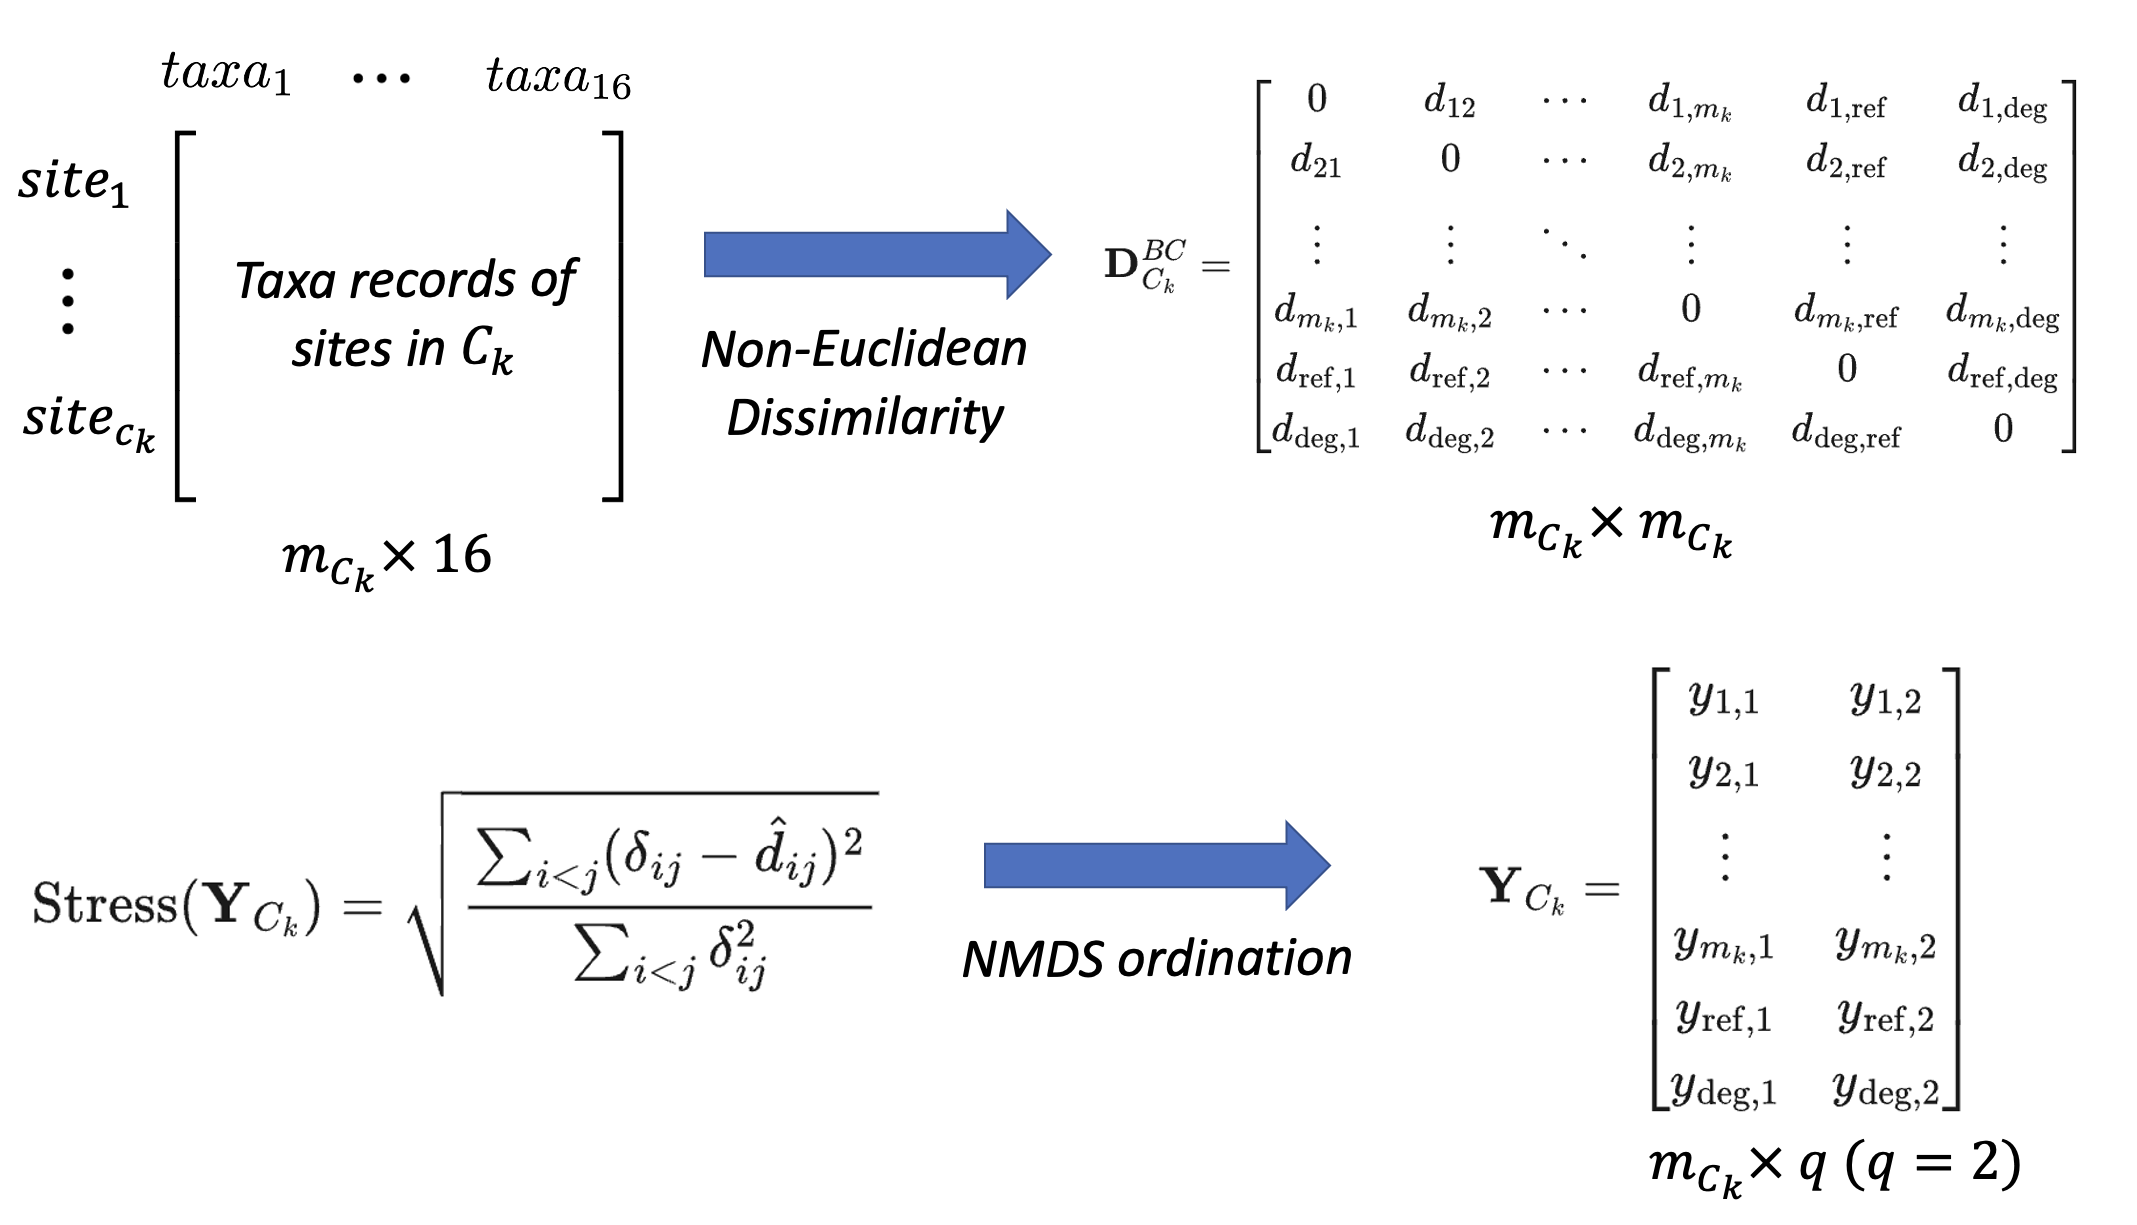
\includegraphics[width=0.73\textwidth]
    {images/slides_13.png}
\end{figure}
\end{frame}


% page 15
\begin{frame}{NMDS to embed the non-Euclidean Bray-Curtis Dissimilarity into a 
    Euclidean-geometry space of lower dimensions}
    \begin{figure}
        \centering
        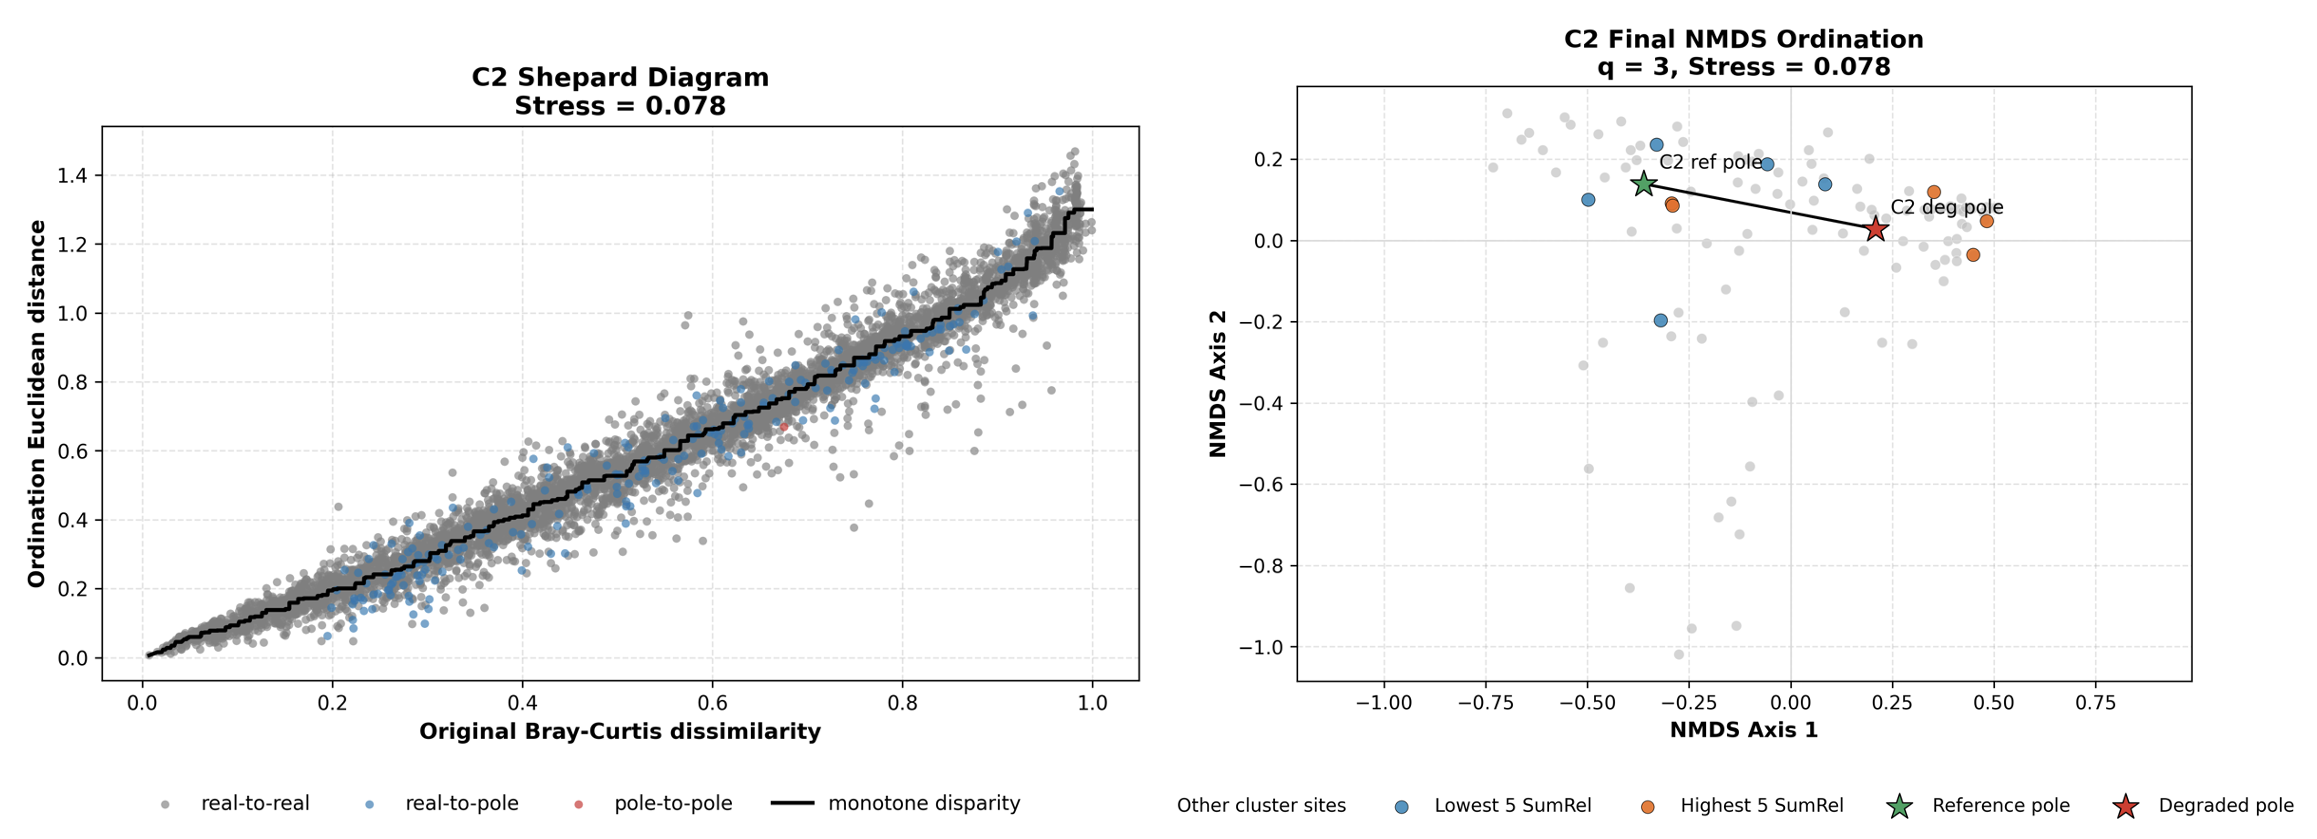
\includegraphics[width=0.9\textwidth]
        {images/slides_15_2.png}
    \end{figure}
\end{frame}


% page 16
\begin{frame}{NMDS Results Across Community Types}
    \begin{figure}
        \centering
        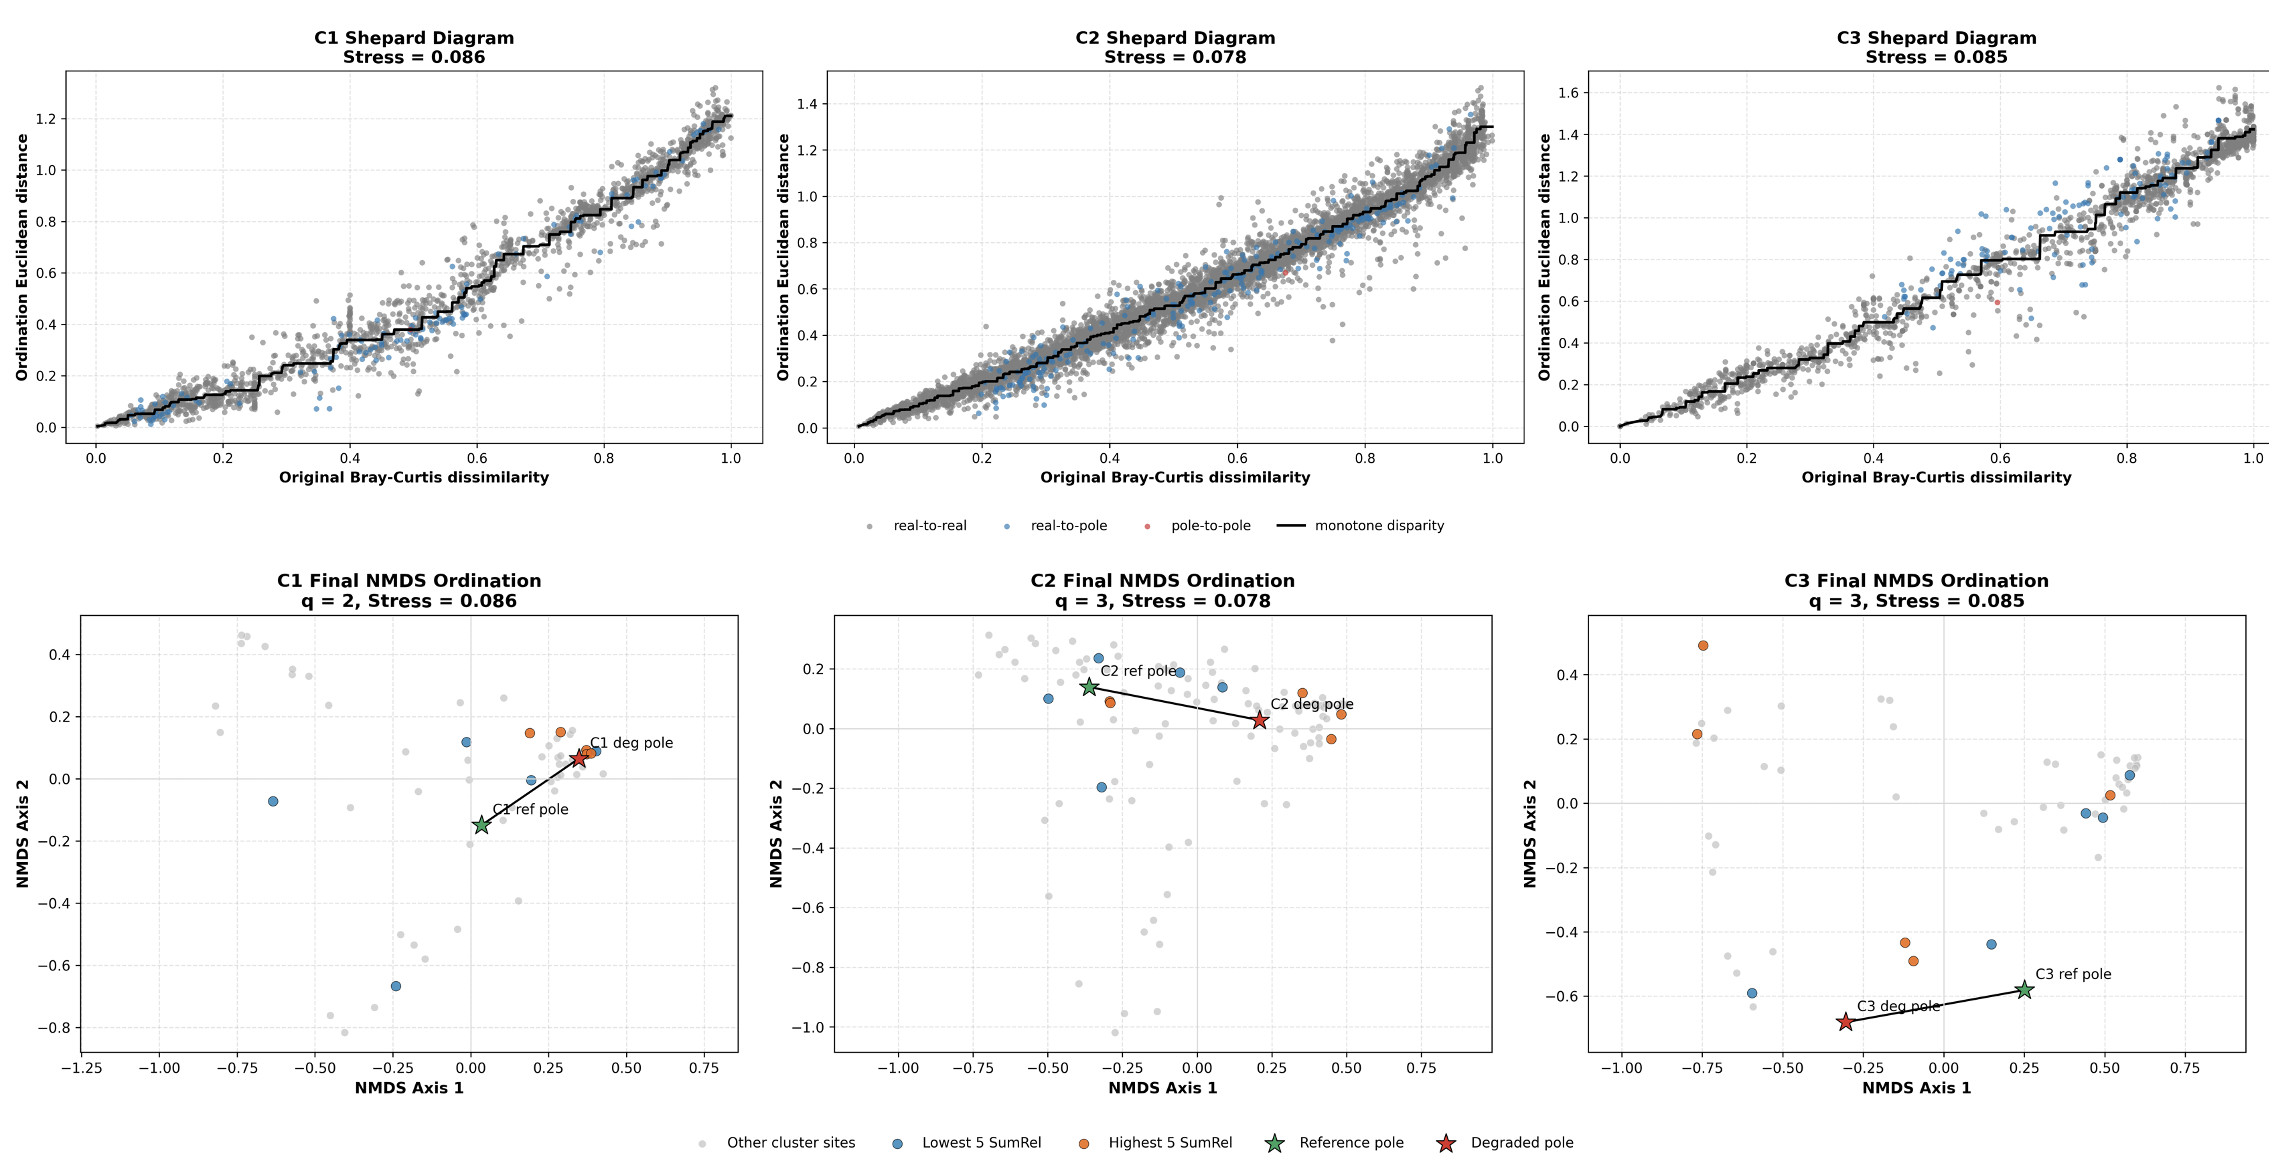
\includegraphics[width=0.9\textwidth]
        {images/slides_16_2.png}
    \end{figure}
\end{frame}


% page 17
\begin{frame}{Projection (ZCI) of Sites onto Pole-Direction to Quantify Community Dissimilarity}
    \begin{figure}
        \centering
        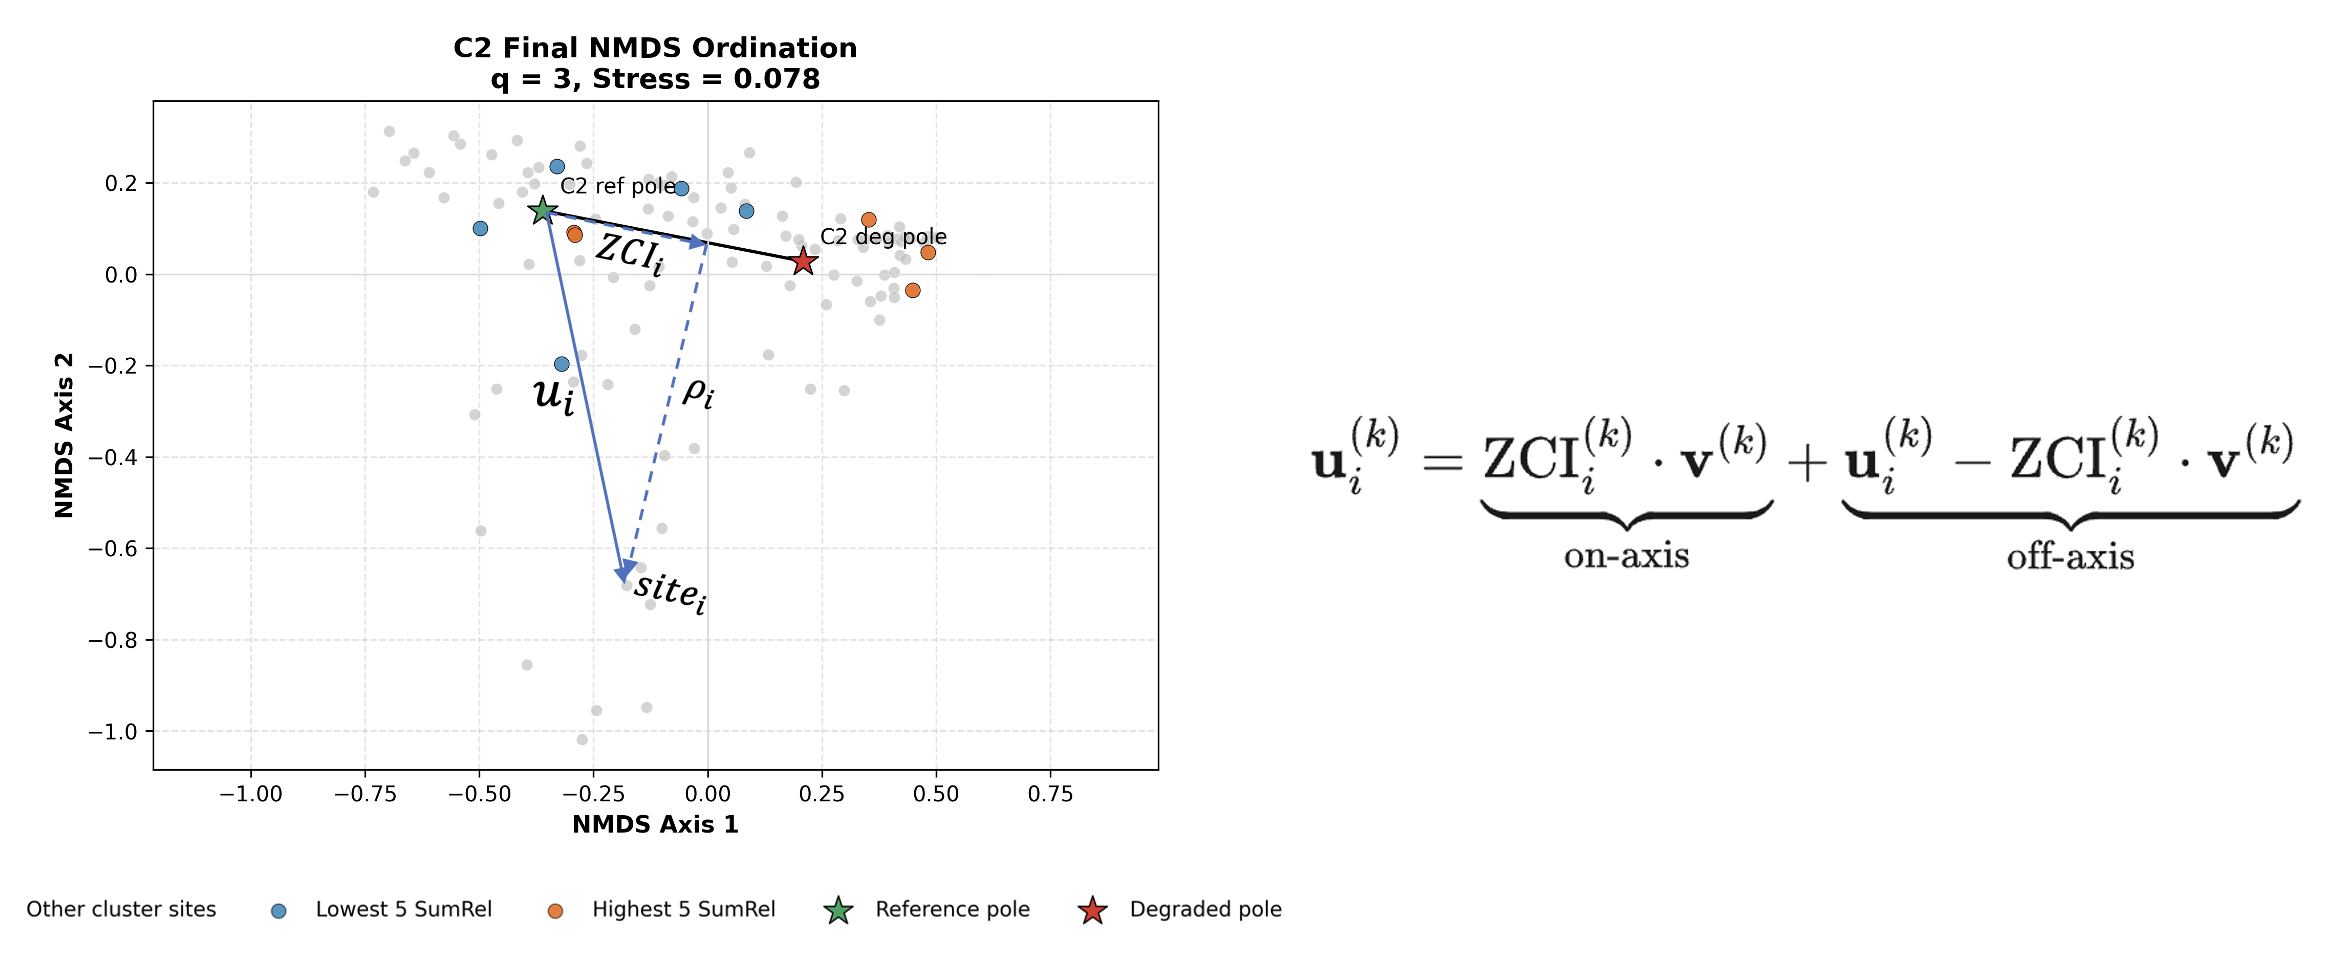
\includegraphics[width=0.9\textwidth]
        {images/slides_17.png}
    \end{figure}
\end{frame}

% page 18
\begin{frame}{Piecewise Quantile Regression between ZCI and Contamination Score}
    \begin{figure}
        \centering
        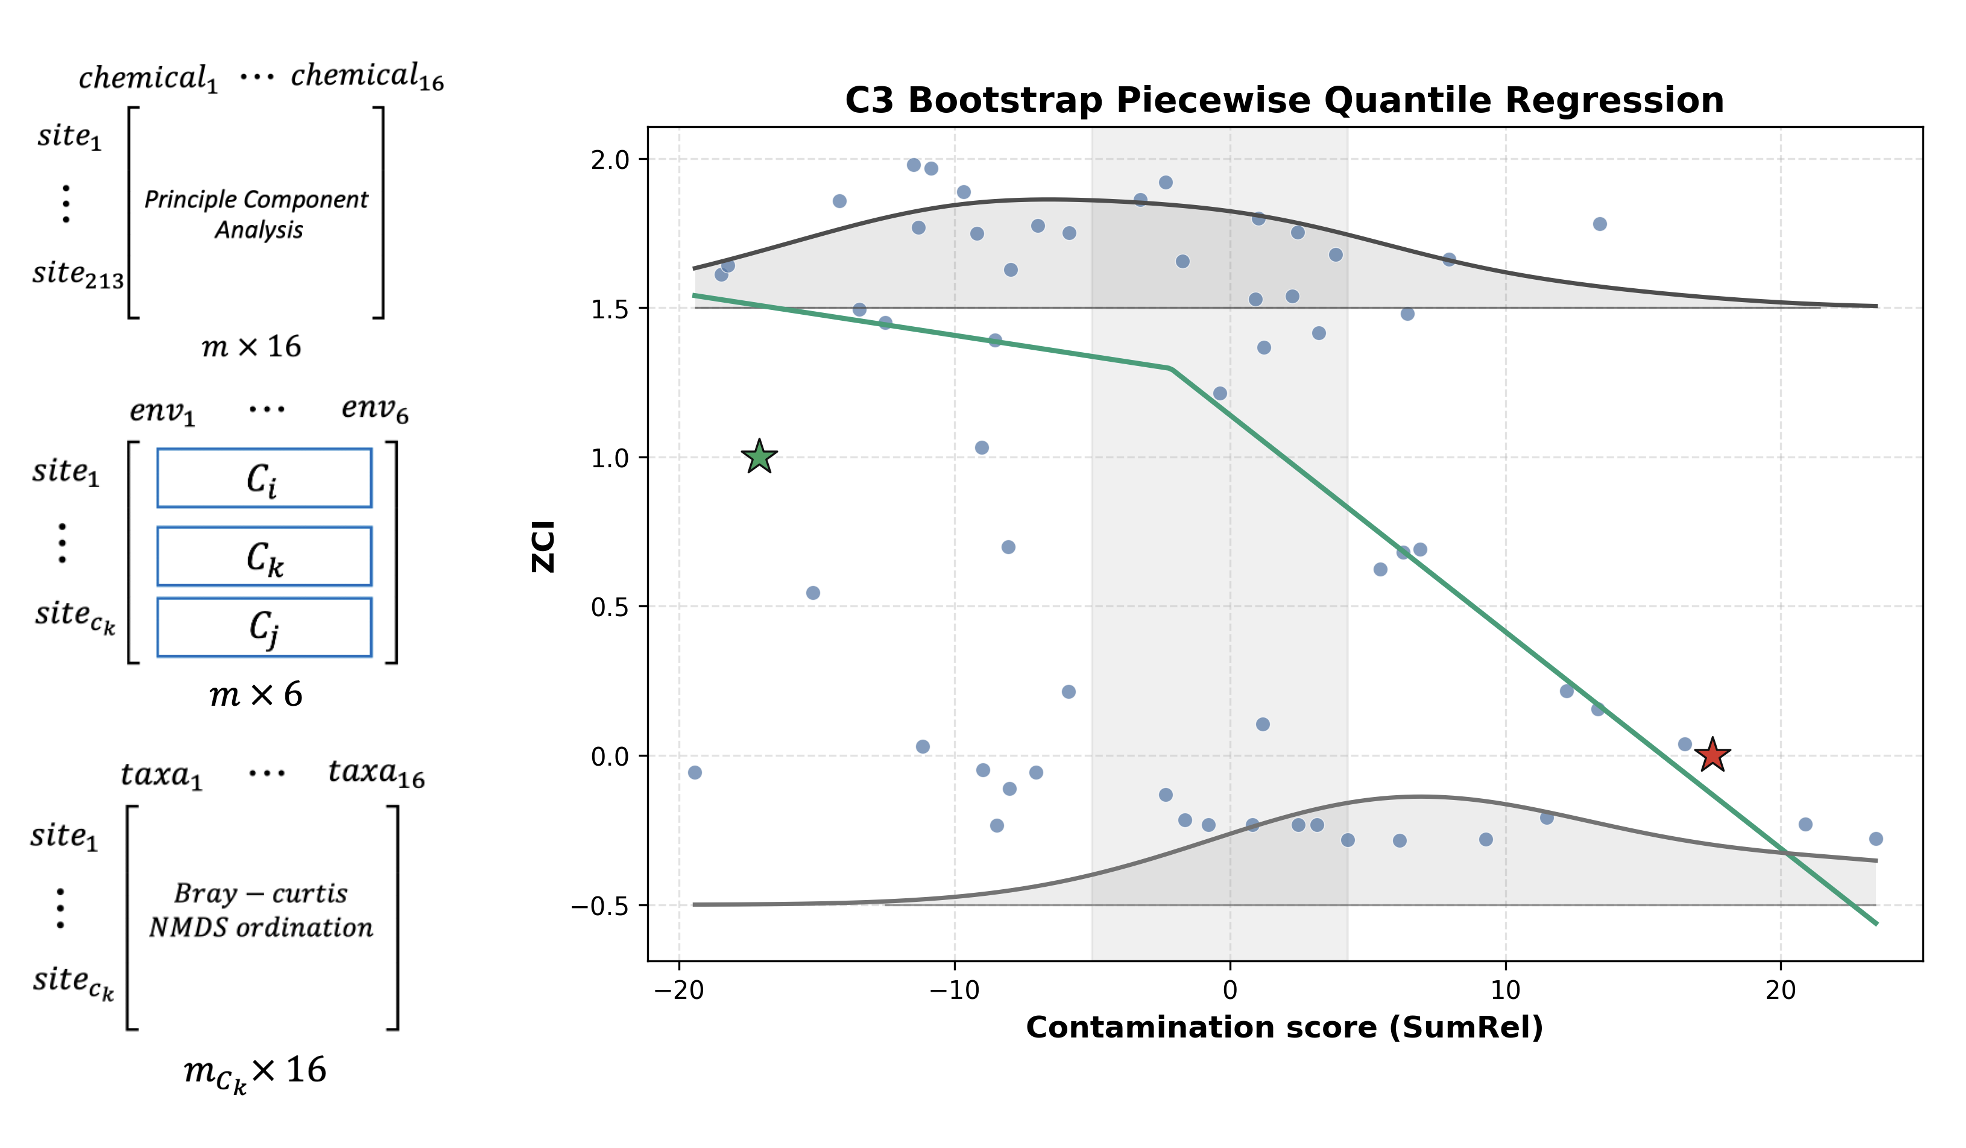
\includegraphics[width=0.85\textwidth]
        {images/slides_18.png}
    \end{figure}
\end{frame}

\end{document}

